\documentclass[11pt]{article}
\usepackage{amsmath,amssymb,amsthm}
\usepackage[margin=1in]{geometry}
% \usepackage{enumitem}
\usepackage{graphicx}

\newcommand{\tophalf}[1]{\includegraphics[width=\textwidth,trim={0 7.5cm 0 0},clip]{#1}}
\newcommand{\topleft}[2]{\includegraphics[width=#1\textwidth,trim={0 7.5cm 19cm 0},clip]{#2}}
\newcommand{\topmiddle}[2]{\includegraphics[width=#1\textwidth,trim={9.5cm 7.5cm 9.5cm 0},clip]{#2}}
\newcommand{\topright}[2]{\includegraphics[width=#1\textwidth,trim={19cm 7.5cm 0 0},clip]{#2}}

\newcommand{\bottomhalf}[1]{\includegraphics[width=\textwidth,trim={0 0 0 7.5cm},clip]{#1}}
\newcommand{\bottomleft}[2]{\includegraphics[width=#1\textwidth,trim={0 0 19cm 7.5cm},clip]{#2}}
\newcommand{\bottommiddle}[2]{\includegraphics[width=#1\textwidth,trim={9.5cm 0 9.5cm 7.5cm},clip]{#2}}
\newcommand{\bottomright}[2]{\includegraphics[width=#1\textwidth,trim={19cm 0 0 7.5cm},clip]{#2}}

% \input{macros}

\begin{document}

We have been investigating when topological persistence is robust to incomplete data.
Specifically, the persistent homology of Vietoris-Rips complexes built from sparse weighted graphs.
In the metric case we can compute the persistent homology of a set of points given a matrix of pairwise distances using state of the art software.
However, computing the persistence of such a matrix requires working with a simplicial complex constructed from the complete metric graph of the point set.
Our hope is that we can get some sense of how to work around missing data by identifying subsets of the complete graph with a persistence diagram close to that of the complete graph.

\begin{figure}[ht]
        \centering
        \topleft{0.4}{figures/722uniform3quarter.pdf}
        \topright{0.4}{figures/722uniform3quarter.pdf}
        \caption{Persistent features of 722 uniformly spaced points sampled from $\mathbb{T}$. The green and red $+$ markers represent expected features at $r=0.3$ and $R-r=0.6$ respectively.}\label{fig:uniform}
\end{figure}

Let $\mathbb{T}_{r,R}$ denote the torus of revolution in $\mathbb{R}^3$ with minor radius $r$ and major radius $R$.
We consider the 1D persistent homology of uniformly and randomly spaced points sampled on $\mathbb{T}_{0.3,0.9}$.
For the sake of notation we will let $\mathbb{T}$ denote $\mathbb{T}_{0.3,0.9}$.

As an initial test we removed edges at random.
Figures~\ref{fig:uniform} and~\ref{fig:random} show the persistence diagrams and representative cycles of uniformly and randomly spaced points sampled from $\mathbb{T}_{0.3,0.9}$.
Figures~\ref{fig:uniform_remove} and~\ref{fig:random_remove} show the effects of removing edges at random.

\begin{figure}[ht]
        \bottomleft{0.32}{figures/722uniform3quarter.pdf}
        \bottomleft{0.32}{figures/722uniformhalf.pdf}
        \bottomleft{0.32}{figures/722uniformquarter.pdf}
        \caption{Persistence diagrams of 722 uniformly spaced points sampled from $\mathbb{T}$ with 25\%, 50\%, and 75\% of the edges removed at random.}\label{fig:uniform_remove}
\end{figure}

Note that in all cases the most prominent feature is retained.
In both the uniform and random case we find that the second most prominent feature, representative of the minor radius can be identified up to 50\% as a peak in the topological noise.

\begin{figure}[ht]
        \centering
        \topleft{0.4}{figures/500random3quarter.pdf}
        \topright{0.4}{figures/500random3quarter.pdf}
        \caption{Persistent features of 500 randomly sampled points from $\mathbb{T}$. The green and red $+$ markers represent expected features at $r=0.3$ and $R-r=0.6$ respectively.}\label{fig:random}
\end{figure}

We then assumed the diagram of the underlying space is known - that is, in the case of $\mathbb{T}$ we know $r=0.3$ and $R=0.9$.
Figures~\ref{fig:uniform_e} and~\ref{fig:random_e} show the effect of only keeping edges $\{p,q\}$ such that $|d(p,q)| < 0$, $|d(p,q)-r| < \epsilon$, or $|d(p,q)-(R-r)| < \epsilon$ for decreasing $\epsilon$.

\begin{figure}[ht]
        \bottomleft{0.32}{figures/500random3quarter.pdf}
        \bottomleft{0.32}{figures/500randomhalf.pdf}
        \bottomleft{0.32}{figures/500randomquarter.pdf}
        \caption{Persistence diagrams of 500 randomly sampled points from $\mathbb{T}_{3,9}$ with 25\%, 50\%, and 75\% of the edges removed at random.}\label{fig:random_remove}
\end{figure}

Figure~\ref{fig:uniform_e} shows the persistence diagrams of four decrasing $\epsilon$ values constructed from ~36\%-18\% of the total number of edges in the 722 point uniform sample.
The full diagram of the uniformly spaced sample took ~64 seconds.
For $\epsilon\approx 0.06$, the maximum value for which both features appear, computing the diagram with 20\% of the edges took ~7.8 seconds.

\begin{figure}[ht]
        \centering
        % 722 points
        % elapsed time: 64.39194748 seconds
        \bottomleft{0.4}{{figures/722uniform6.0}.pdf}
        % _e:	0.10206207261596574
        % 93238 of 260281 edges (~35.8%)
        % elapsed time: 12.710867289 seconds
        \bottomleft{0.4}{{figures/722uniform9.0}.pdf}\\
        % _e:	0.06804138174397717
        % 58488 of 260281 edges (~22.5%)
        % elapsed time: 6.942943824 seconds
        \bottomleft{0.4}{{figures/722uniform10.0}.pdf}
        % _e:	0.06123724356957945
        % 52870 of 260281 edges (~20.3%)
        % elapsed time: 7.834110644 seconds
        \bottomleft{0.4}{{figures/722uniform11.0}.pdf}
        % _e:	0.05567022142689041
        % 45962 of 260281 edges (~17.7%)
        % elapsed time: 7.518238489 seconds
        \caption{Persistence diagrams of 722 uniformly spaced points sampled from $\mathbb{T}$ with $\epsilon\approx0.1,0.07,0.6,0.55$ respectively.}\label{fig:uniform_e}
\end{figure}

Figure~\ref{fig:random_e} shows the persistence diagrams of four decrasing $\epsilon$ values constructed from ~43\%-24\% of the total number of edges in the random sample.
The full diagram of the random spaced sample took ~28 seconds.
For $\epsilon\approx 0.09$, the maximum value for which both features appear, computing the diagram with ~24\% of the edges took ~6.7 seconds.

In both cases we see that for the last $\epsilon$ value the feature whose death depends on the presence of the longest edges does not die, resulting in a diagram which is not immediately representative of the underlying space.
One direction for future would be to work around this issue however, this experiment is useful primarily as a proof-of-concept.
In practice the diagram of the underlying space is often not known.

\begin{figure}[ht]
        \centering
        % 500 points
        % elapsed time: 28.593911778 seconds
        \bottomleft{0.32}{{figures/500random5.0}.pdf}
        % _e:	0.12247448713915889
        % 53104 of 124750 edges (~42.6%)
        % elapsed time: 9.648665505 seconds
        \bottomleft{0.32}{{figures/500random7.0}.pdf}
        % _e:	0.08748177652797064
        % 38855 of 124750 edges (~31.1%)
        % elapsed time: 6.663576161 seconds
        \bottomleft{0.32}{{figures/500random9.0}.pdf}
        % _e:	0.06804138174397717
        % 30128 of 124750 edges (~24.2%)
        % elapsed time: 5.90712126 seconds
        \caption{Persistence diagrams of 500 points randomly sampled from $\mathbb{T}$ with $\epsilon\approx 0.123,0.087,0.068$ respectively.}\label{fig:random_e}
\end{figure}


Moving forward we would like to use these observations to explore ways to manipulate and simplifies input such as distance matrices common among state of the art persistence software to implement approximation schemes such as sparse filtrations and geometric spanners.
Our hope is that methods that are robust to the absence and manipulation of metric information can be naturally applied to non-metric data.

% \begin{figure}[ht]
%         \centering
%         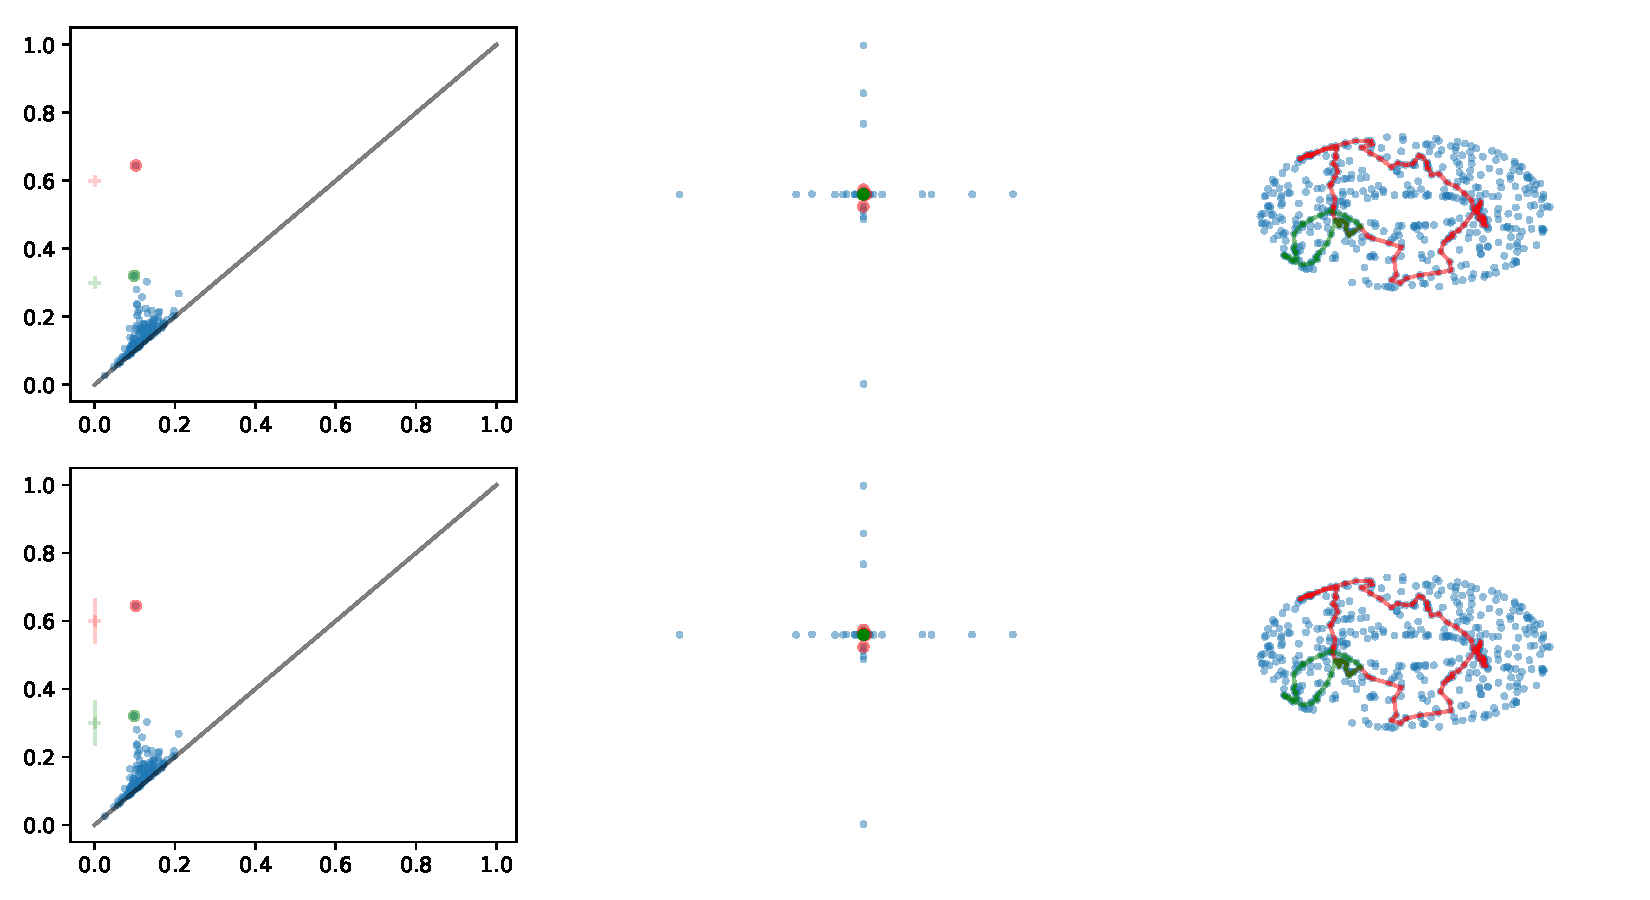
\includegraphics[width=\textwidth]{{figures/500random5.0}.pdf}
%         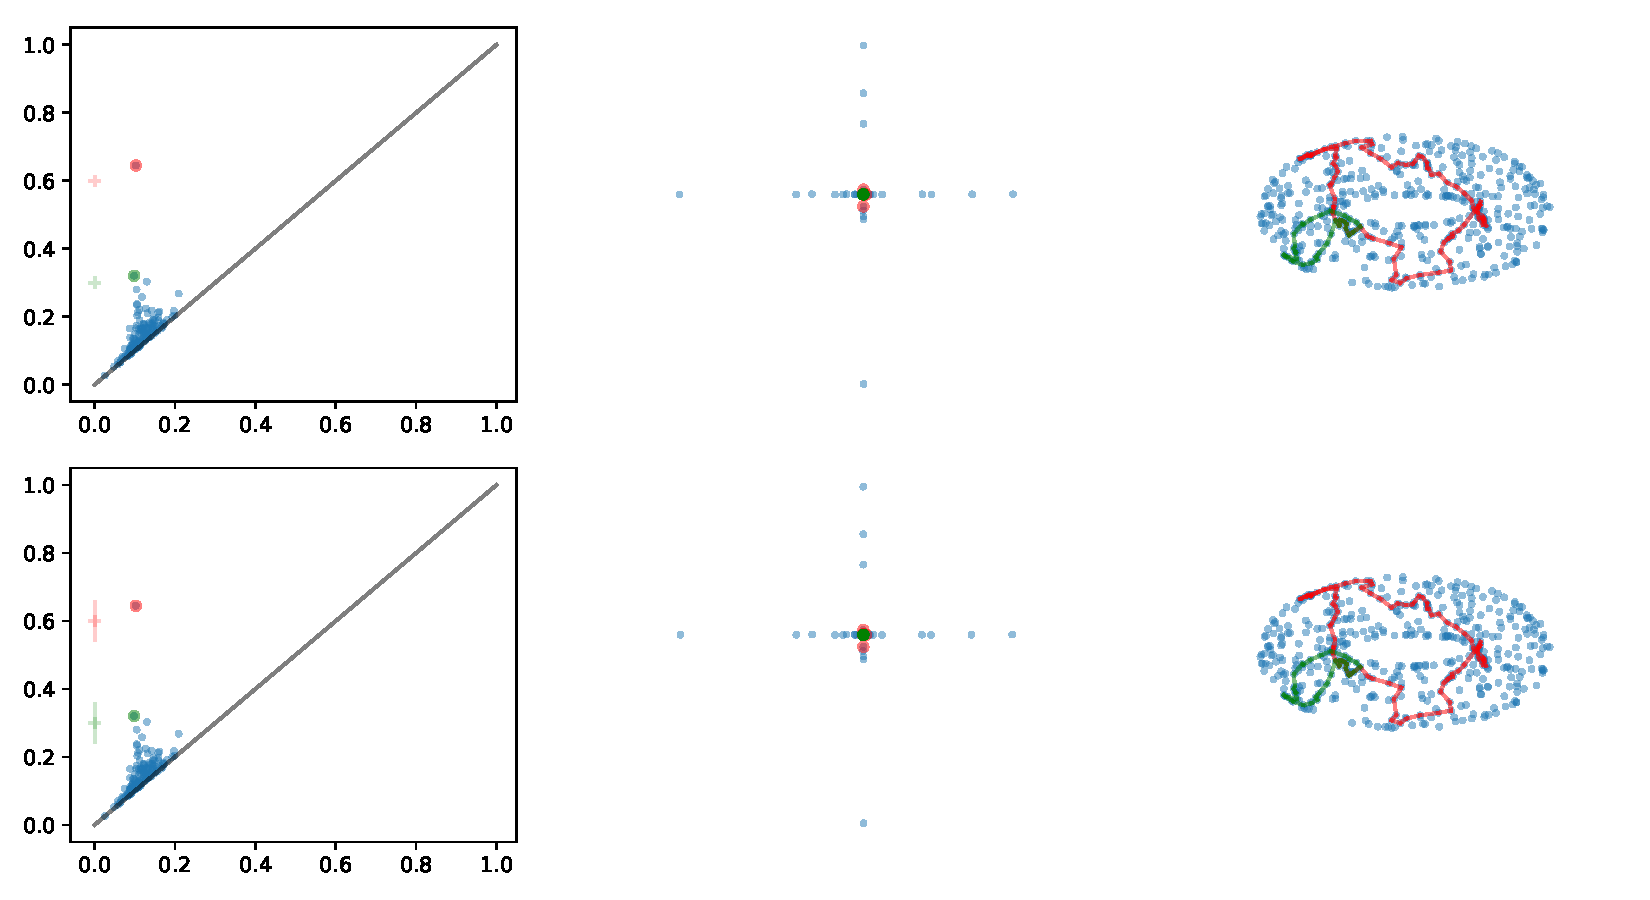
\includegraphics[width=\textwidth]{{figures/500random5.5}.pdf}
%         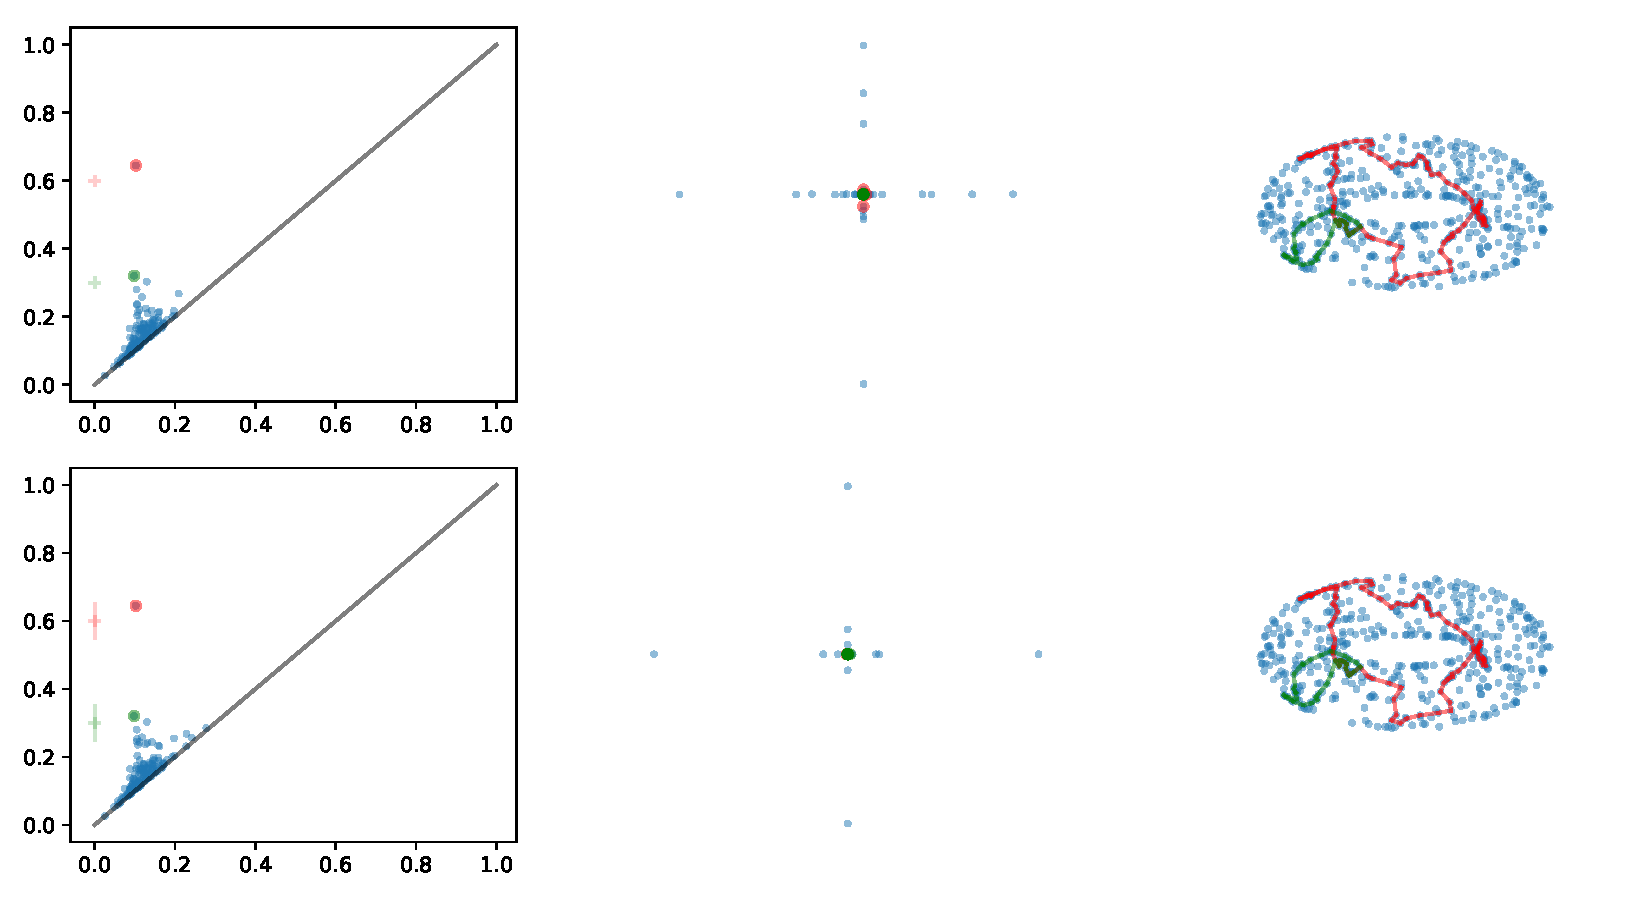
\includegraphics[width=\textwidth]{{figures/500random6.0}.pdf}
%         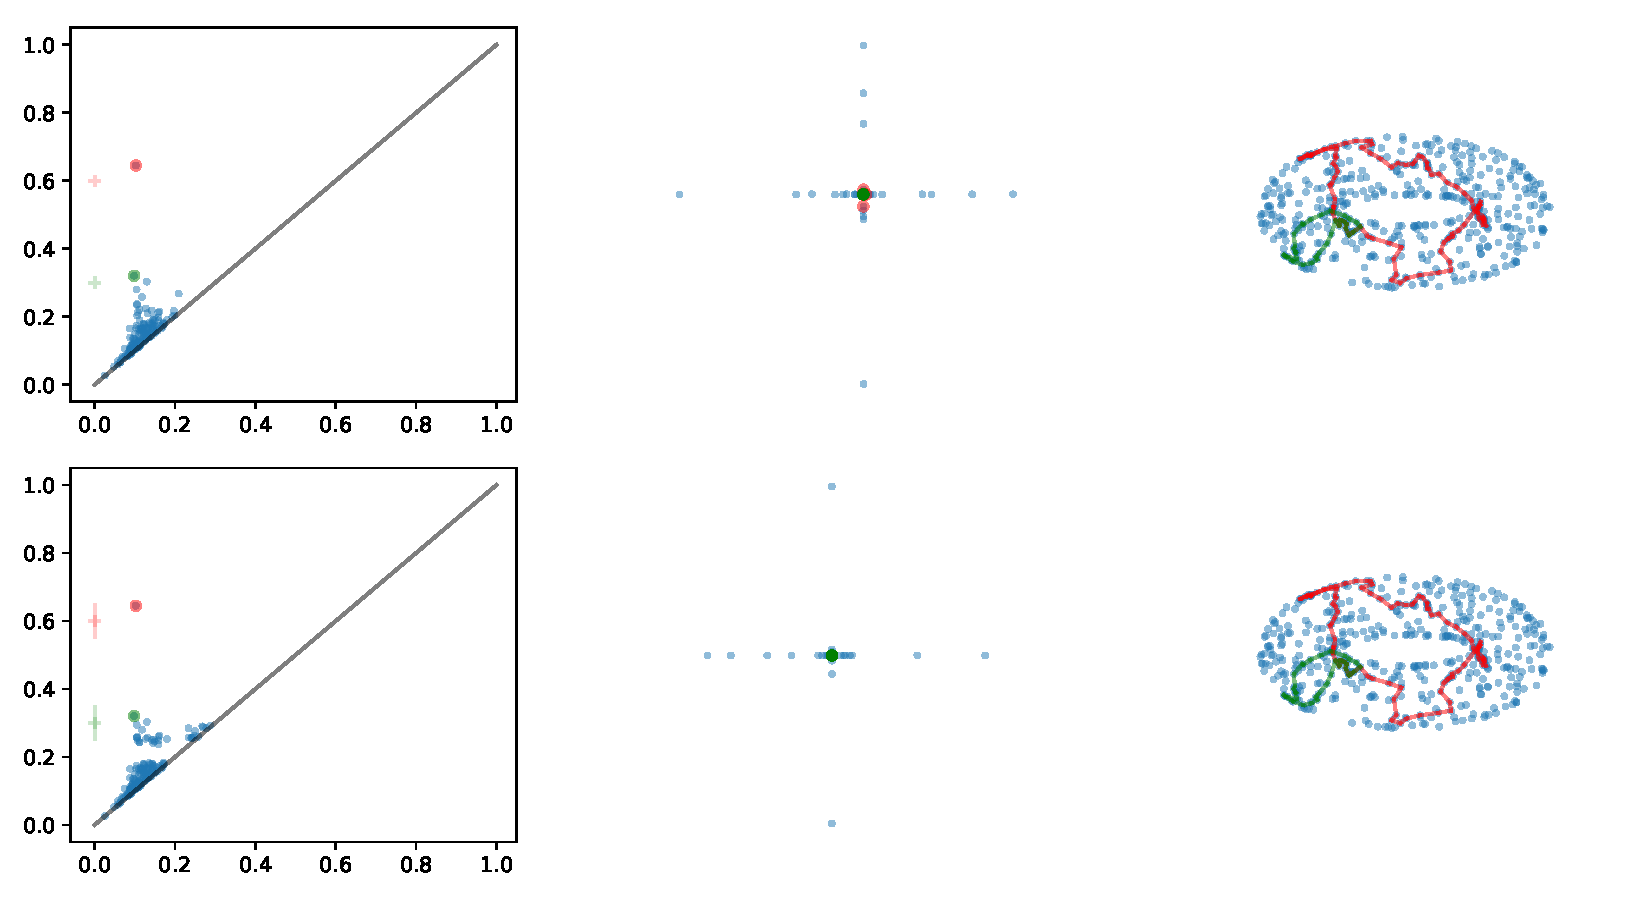
\includegraphics[width=\textwidth]{{figures/500random6.5}.pdf}
%         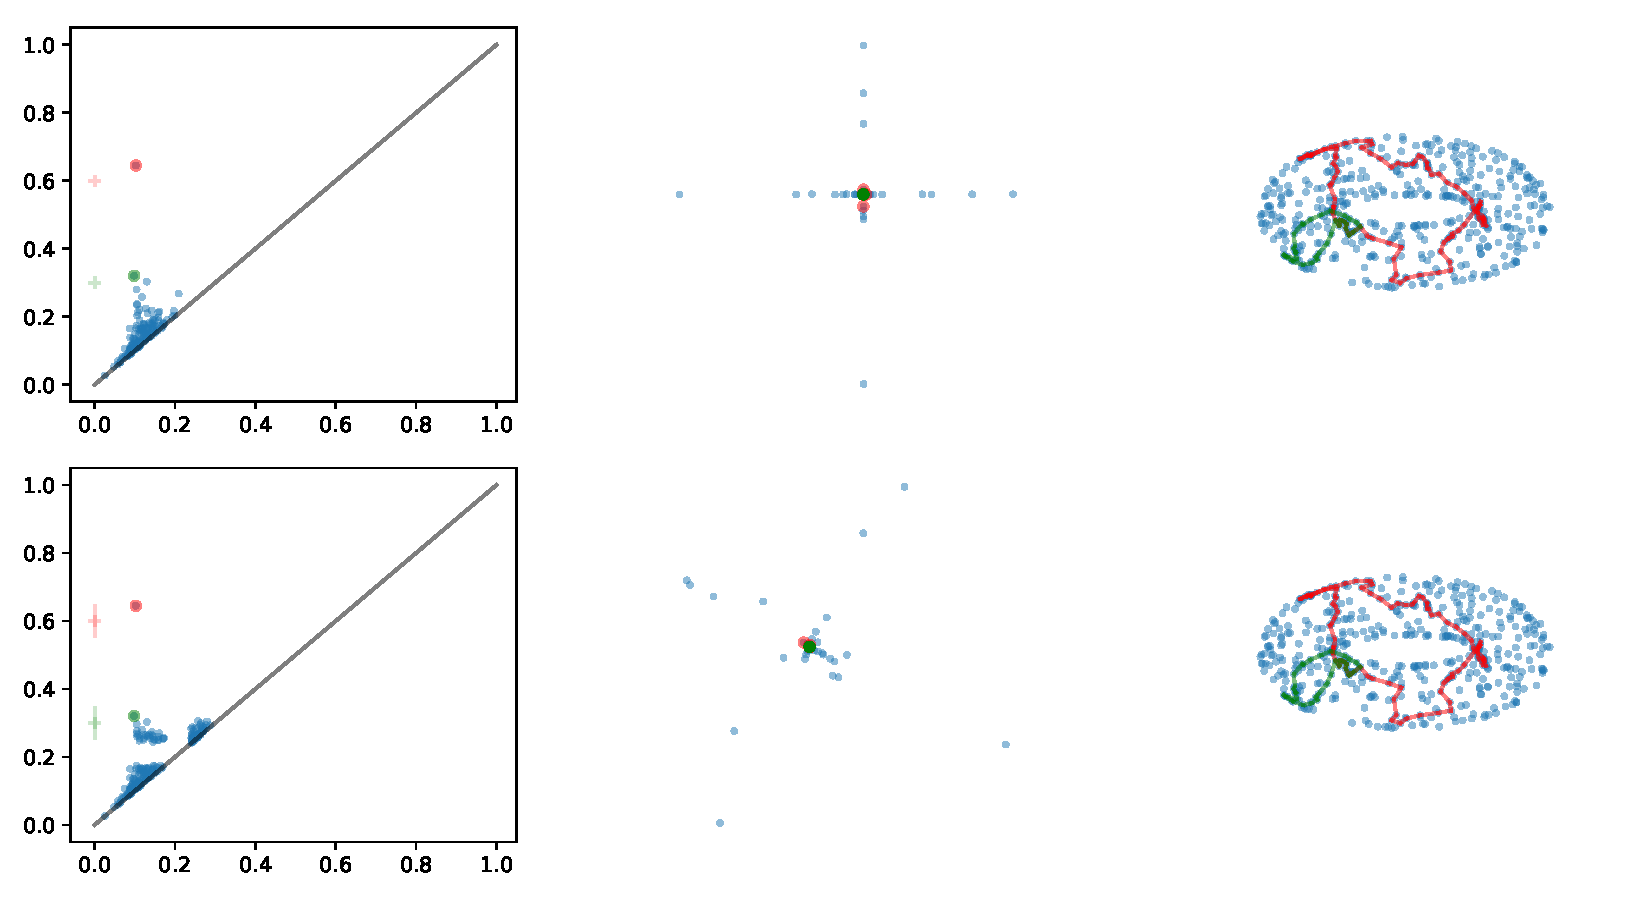
\includegraphics[width=\textwidth]{{figures/500random7.0}.pdf}
%         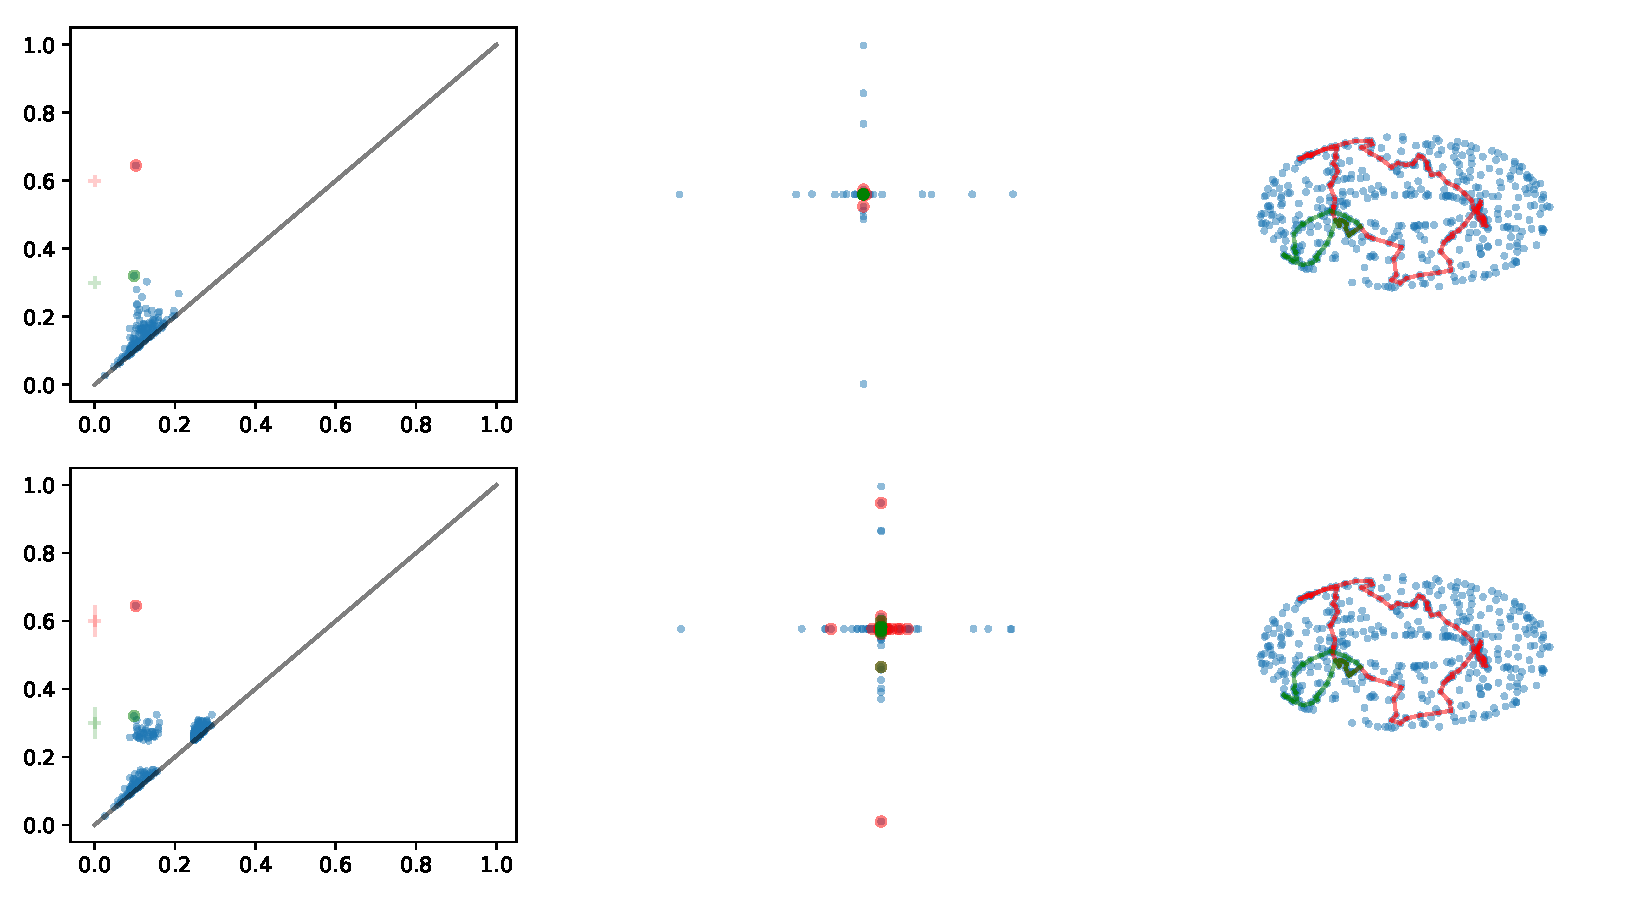
\includegraphics[width=\textwidth]{{figures/500random7.5}.pdf}
%         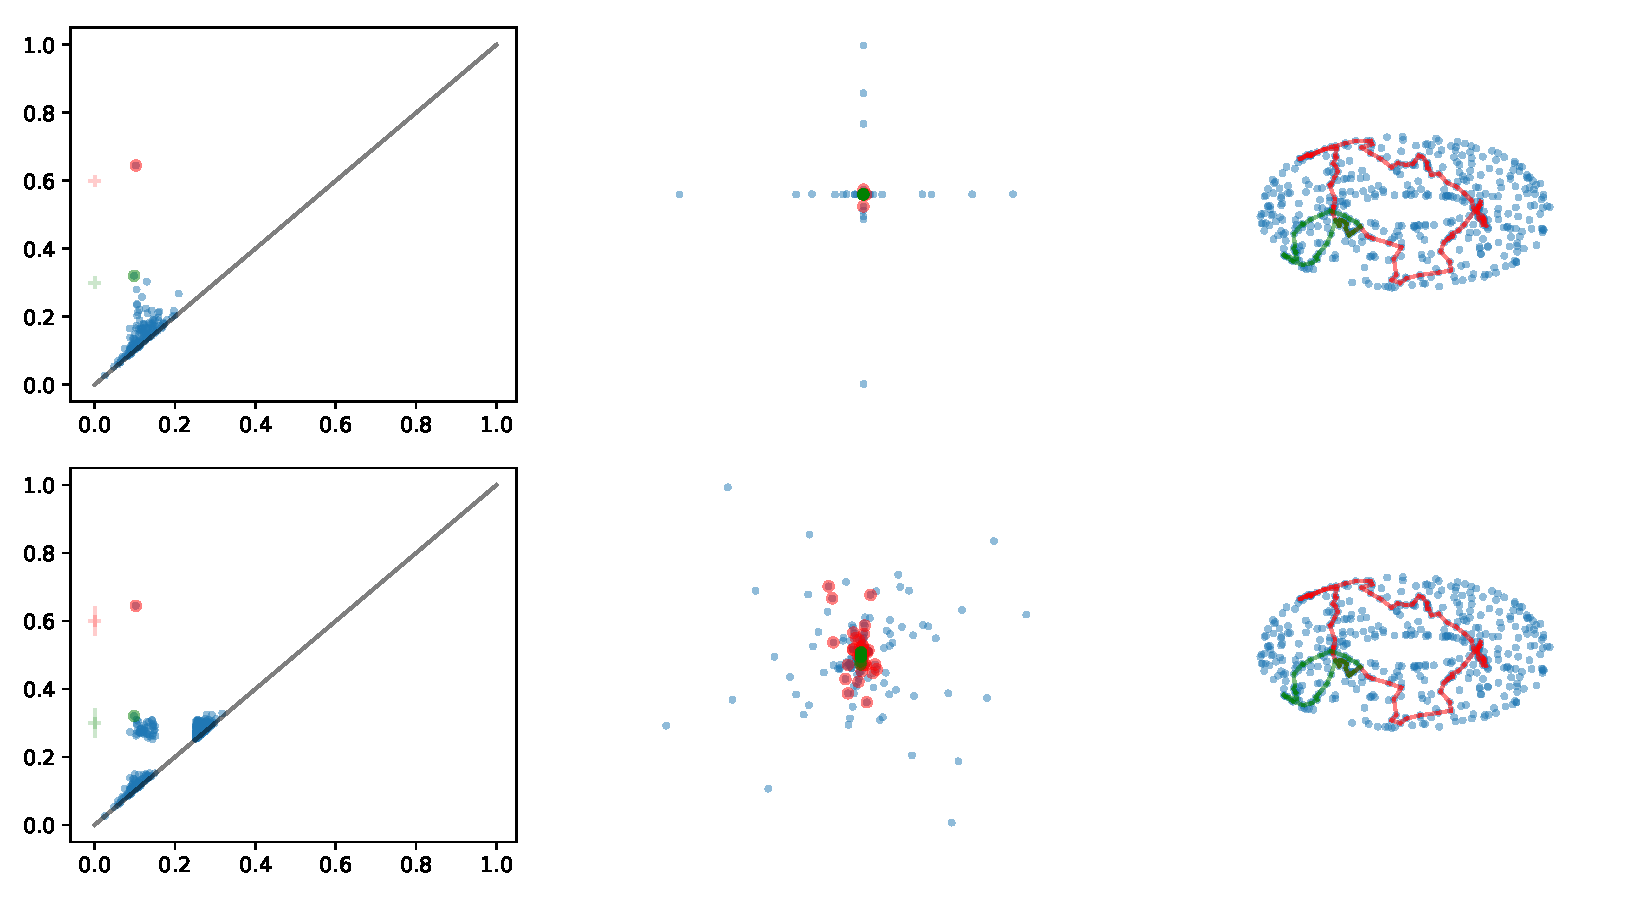
\includegraphics[width=\textwidth]{{figures/500random8.0}.pdf}
%         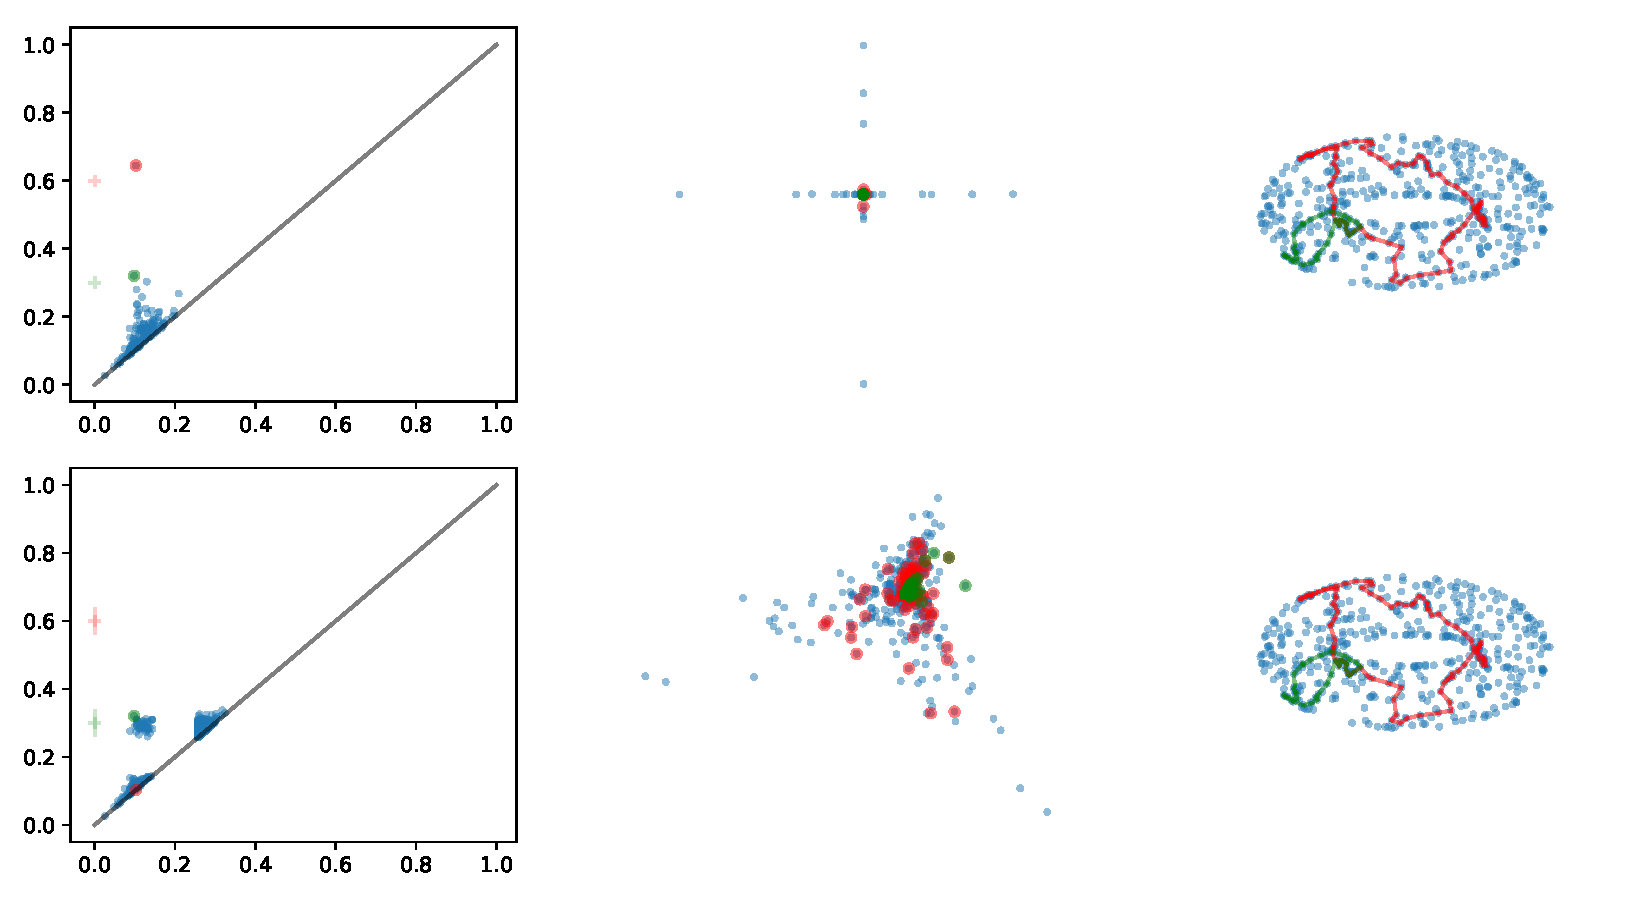
\includegraphics[width=\textwidth]{{figures/500random8.5}.pdf}
%         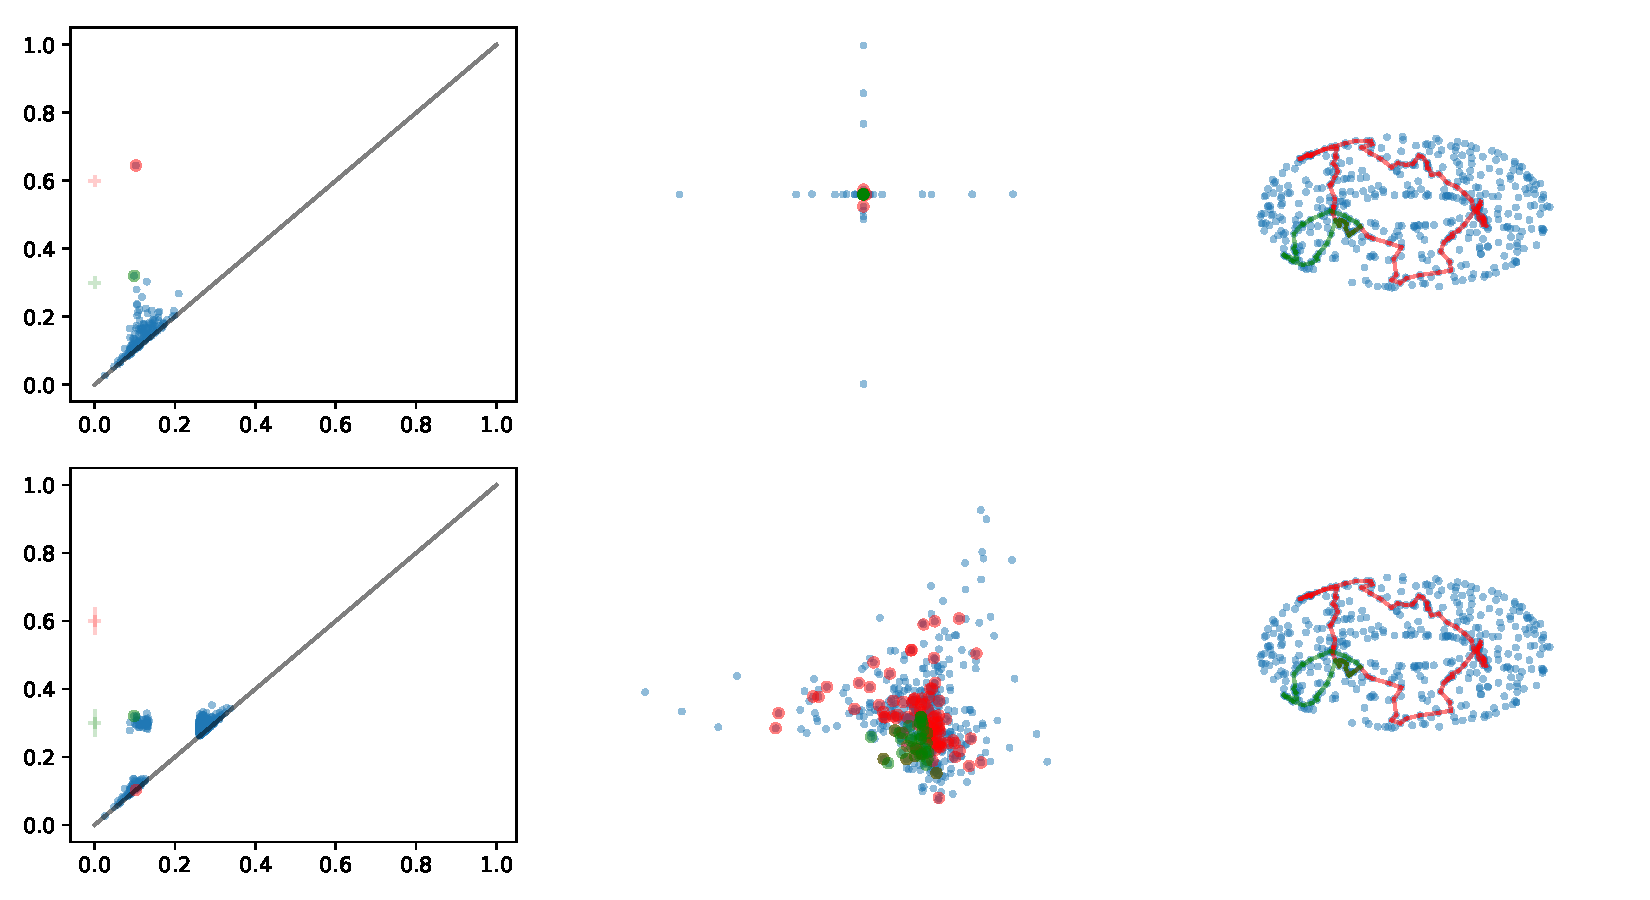
\includegraphics[width=\textwidth]{{figures/500random9.0}.pdf}
%         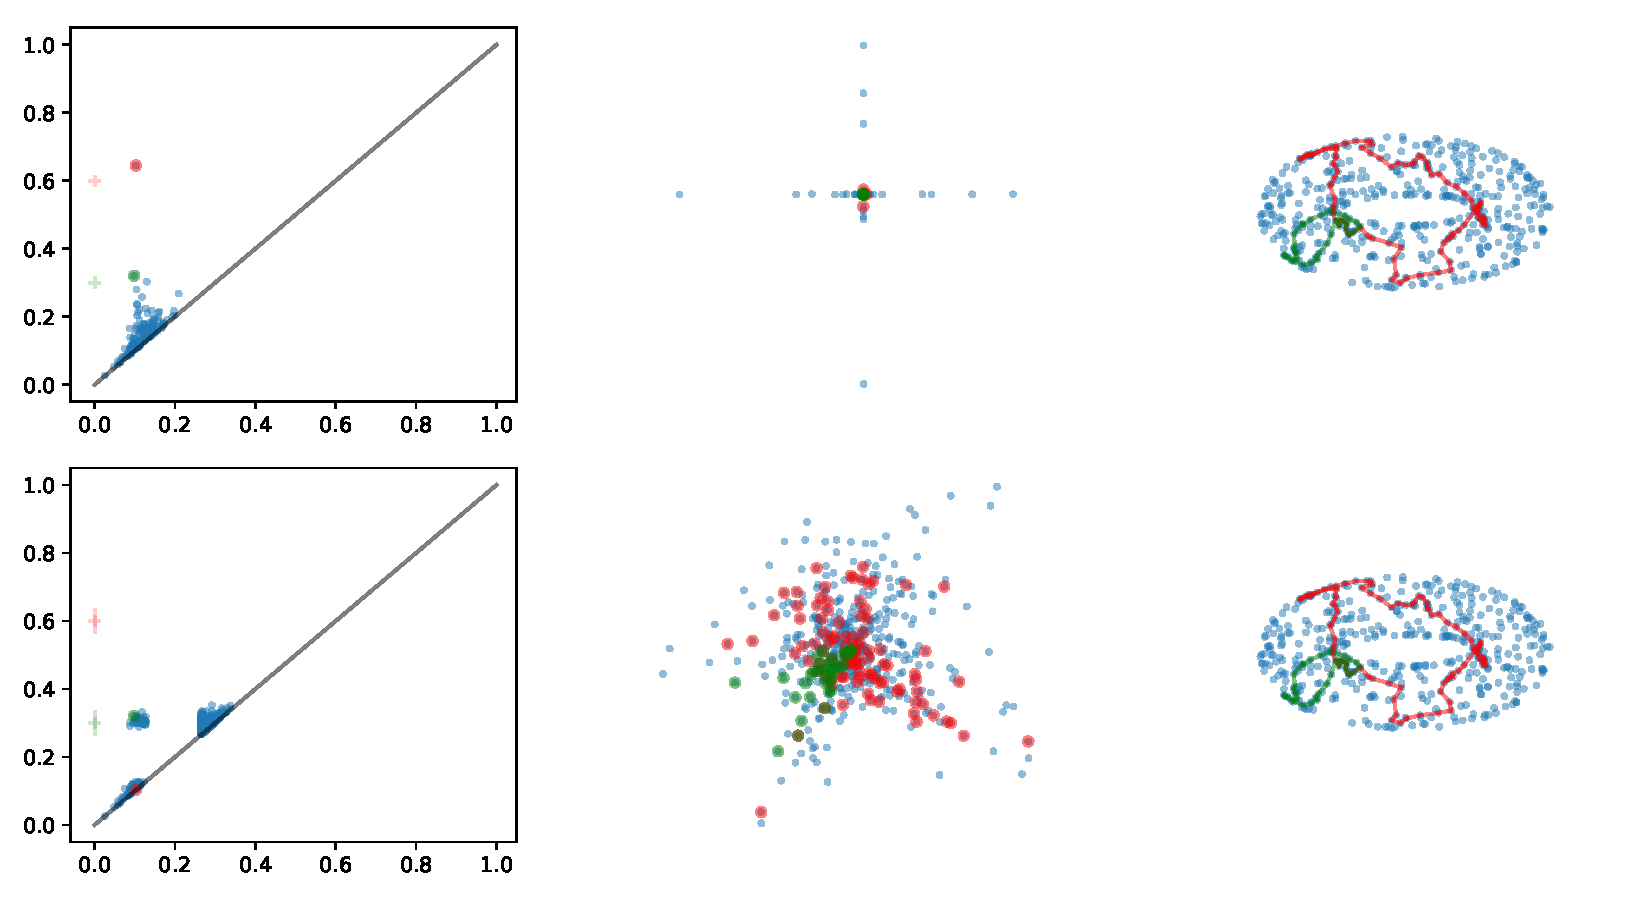
\includegraphics[width=\textwidth]{{figures/500random9.5}.pdf}
%         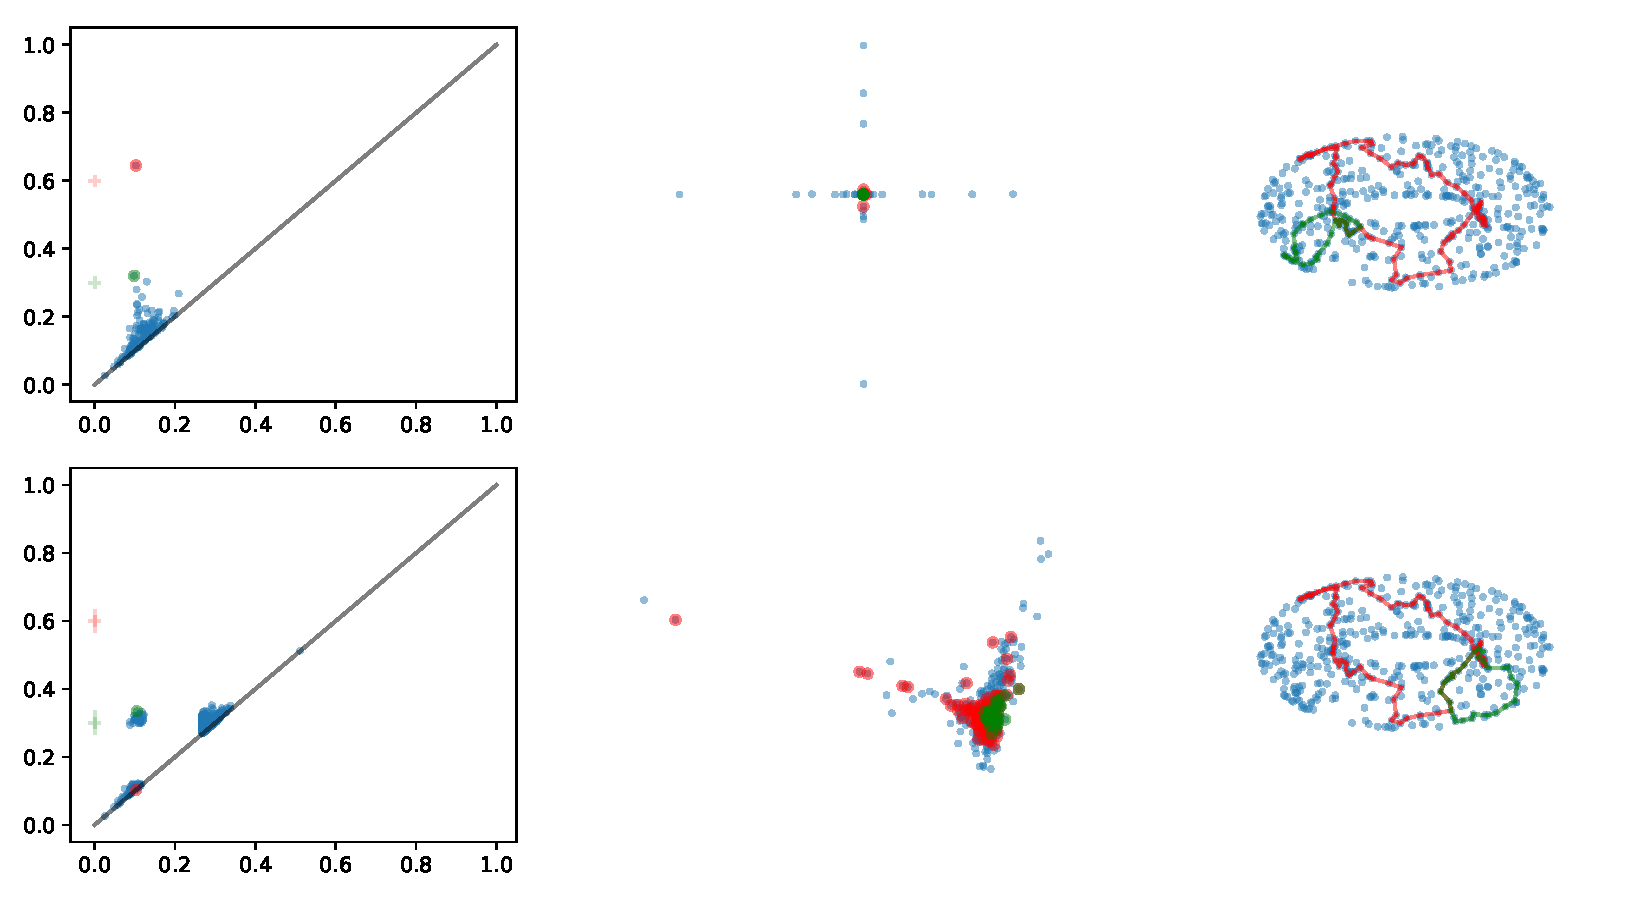
\includegraphics[width=\textwidth]{{figures/500random10.0}.pdf}
%         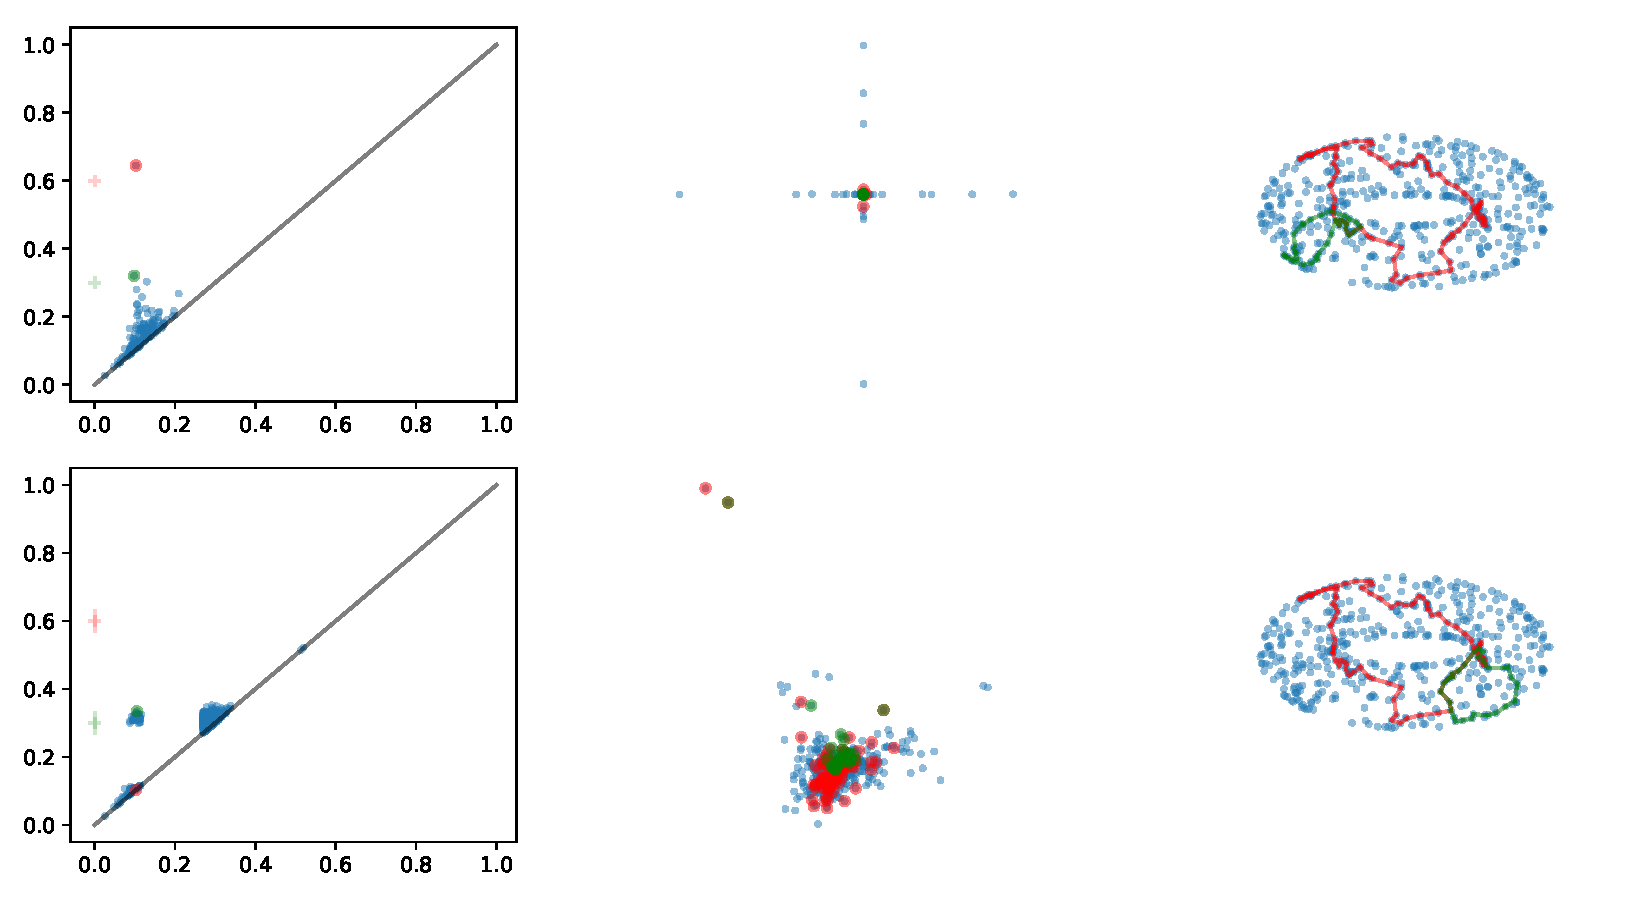
\includegraphics[width=\textwidth]{{figures/500random10.5}.pdf}
%         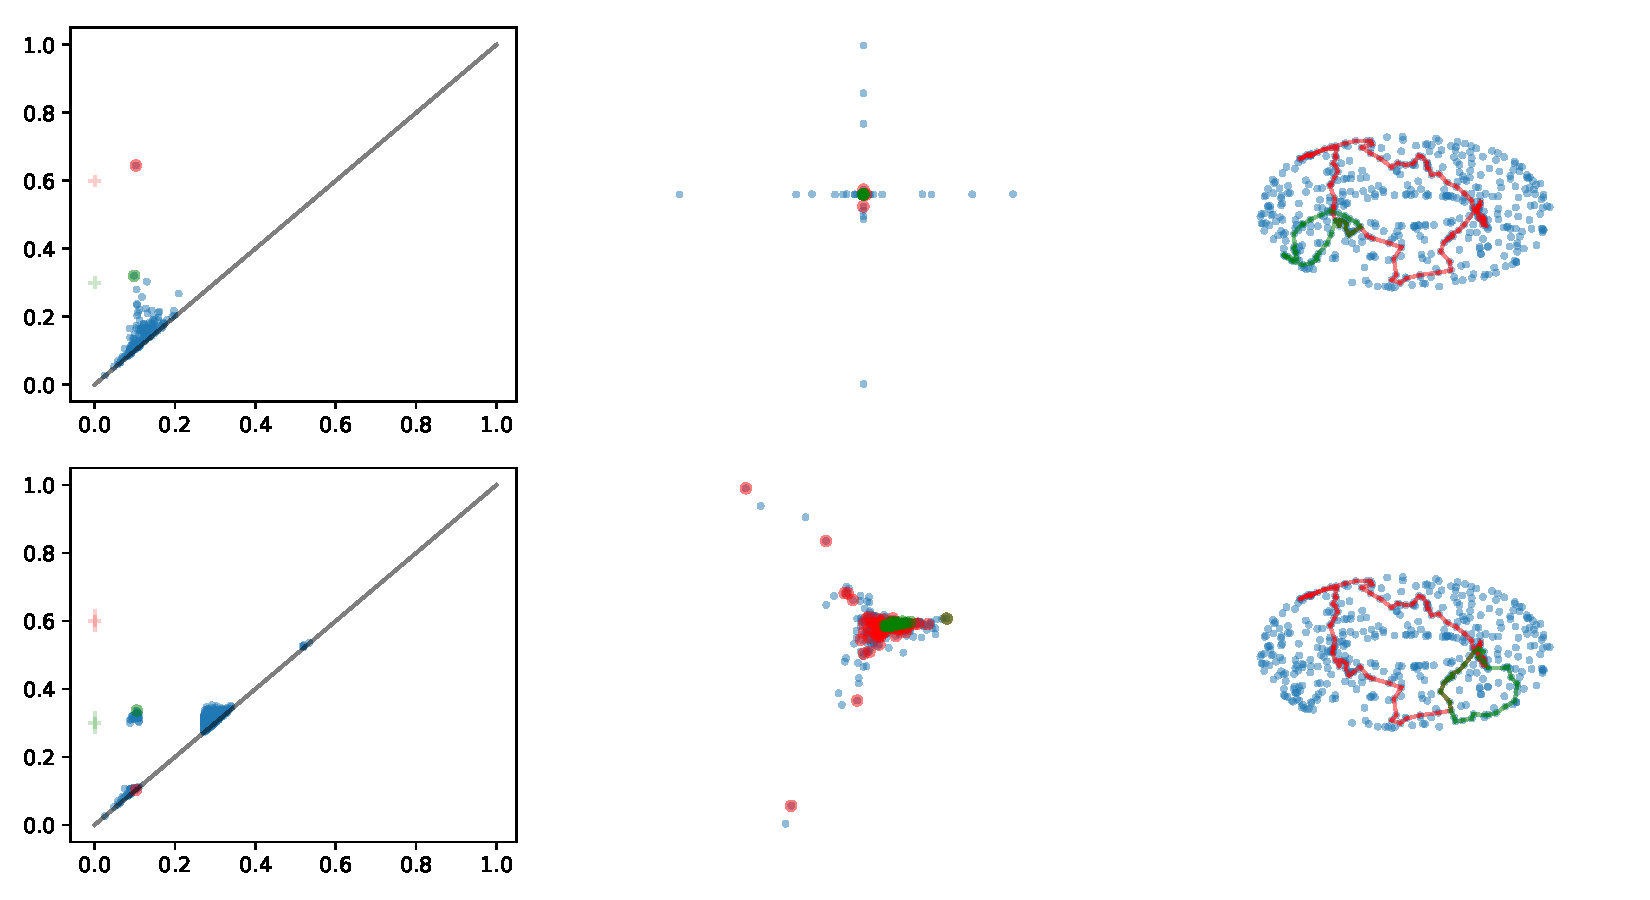
\includegraphics[width=\textwidth]{{figures/500random11.0}.pdf}
%         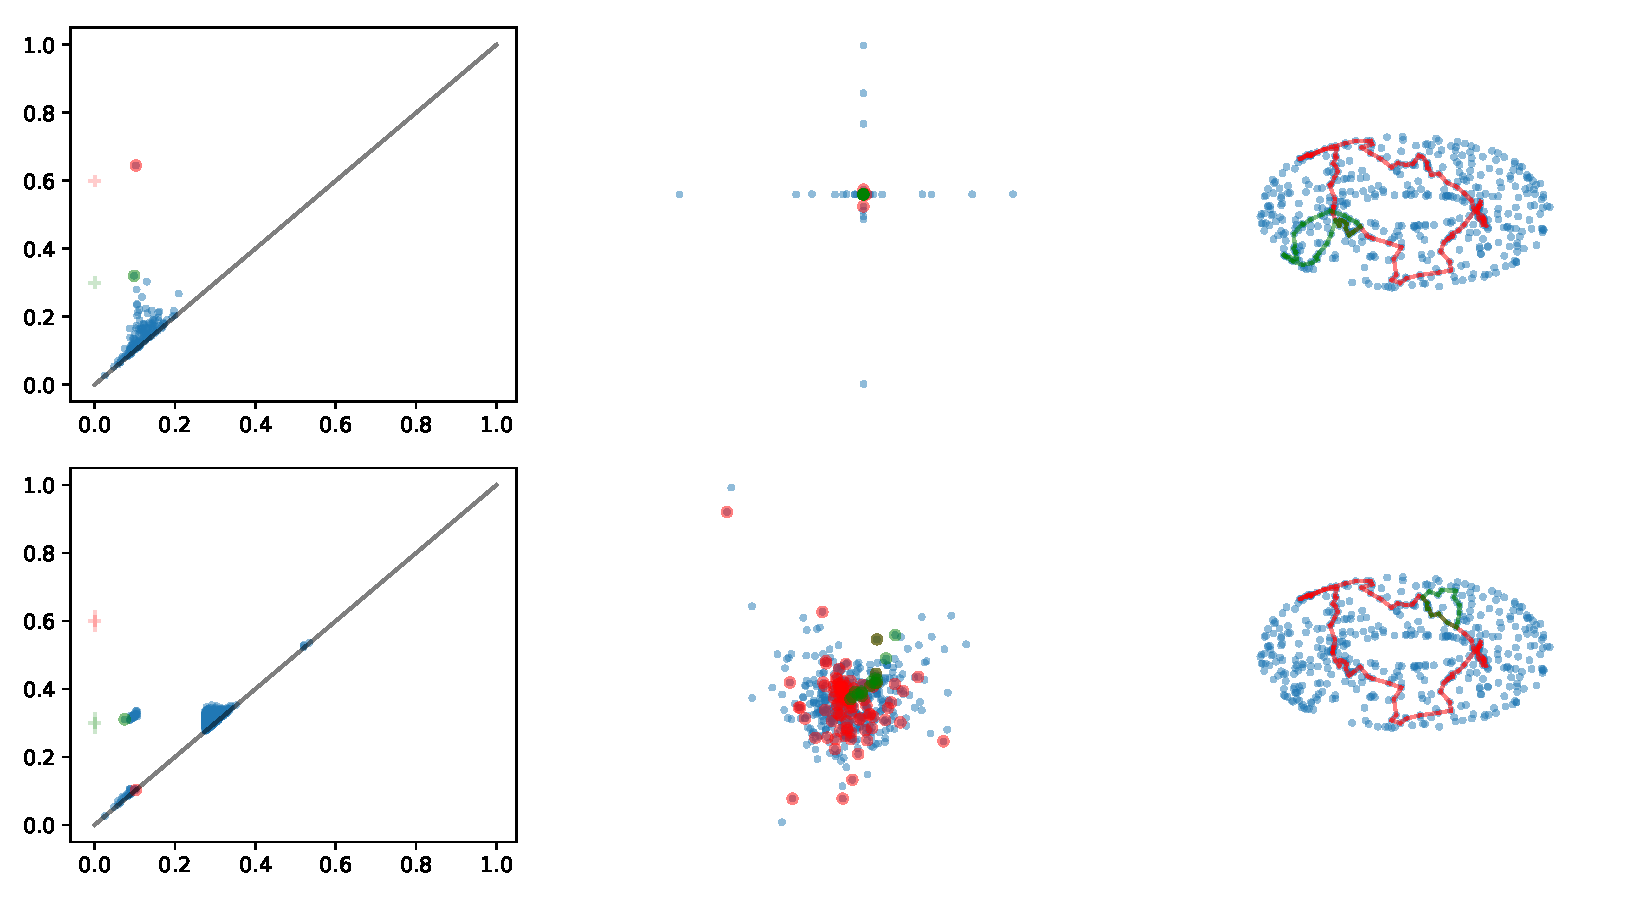
\includegraphics[width=\textwidth]{{figures/500random11.5}.pdf}
%         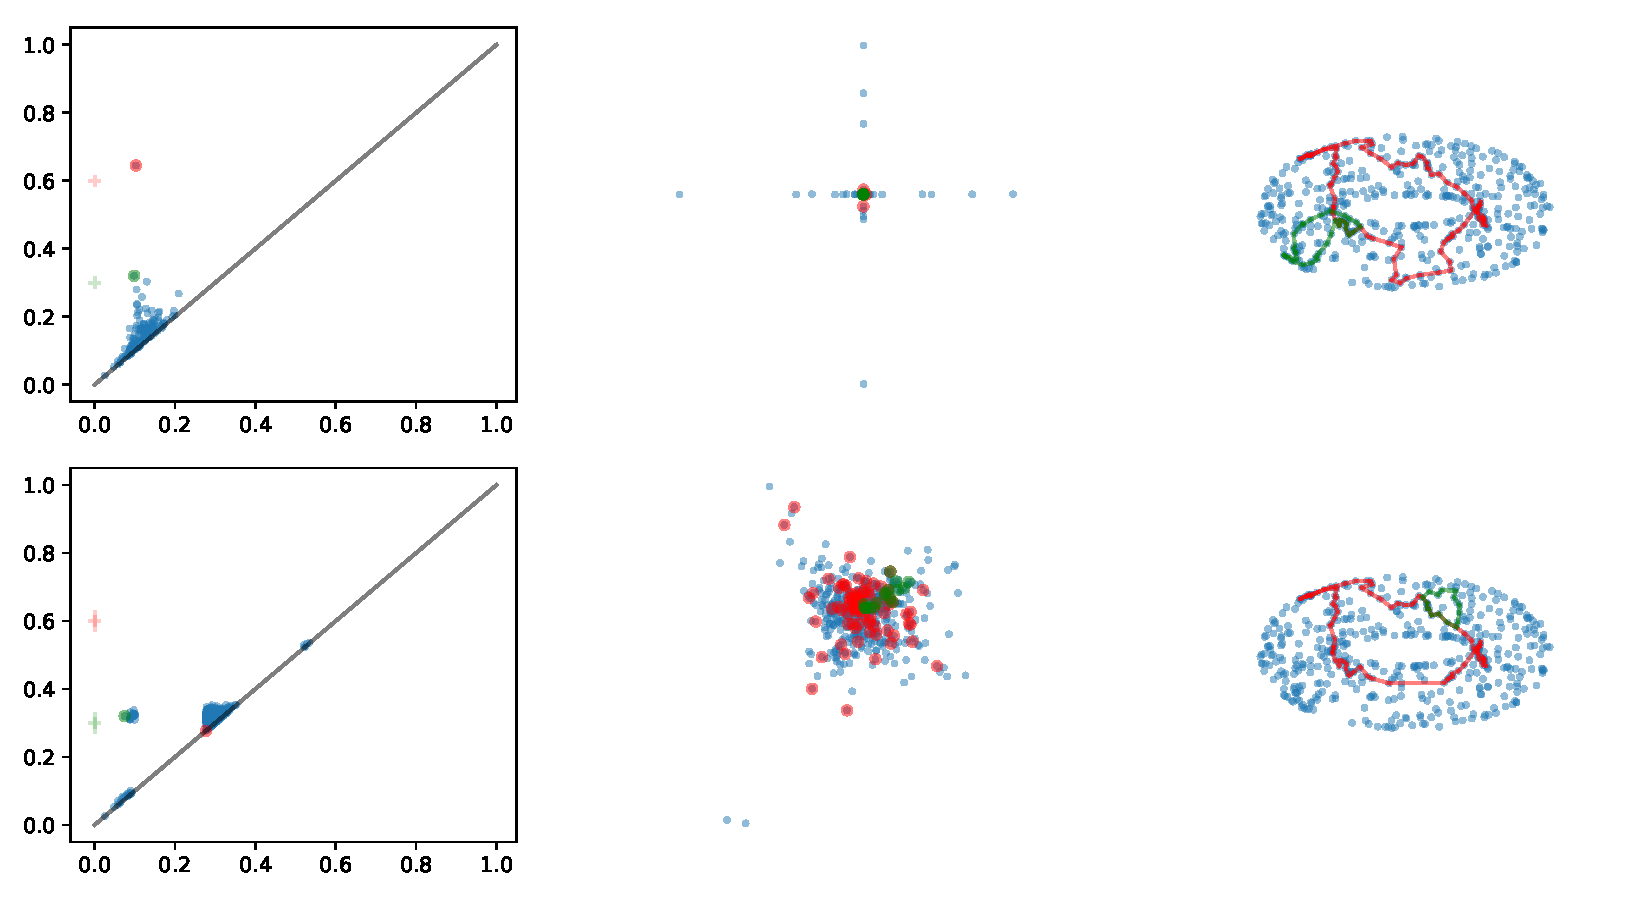
\includegraphics[width=\textwidth]{{figures/500random12.0}.pdf}
%         % \caption{}\label{fig:mdss}
% \end{figure}
% \begin{figure}[ht]
%         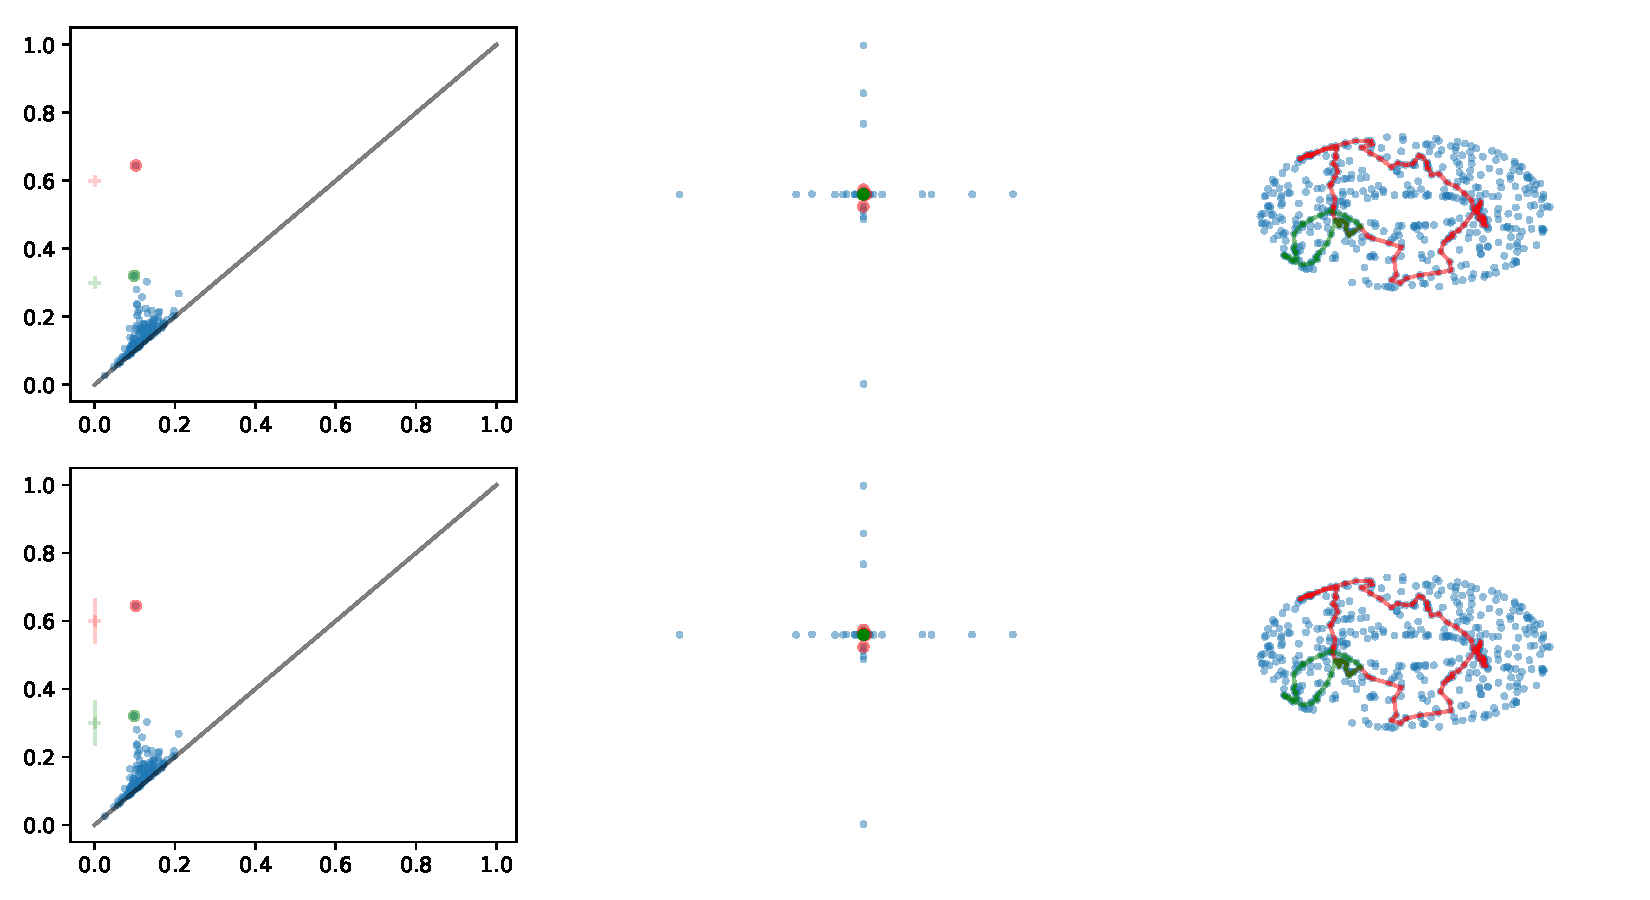
\includegraphics[width=\textwidth]{{figures/500random5.0}.pdf}
%         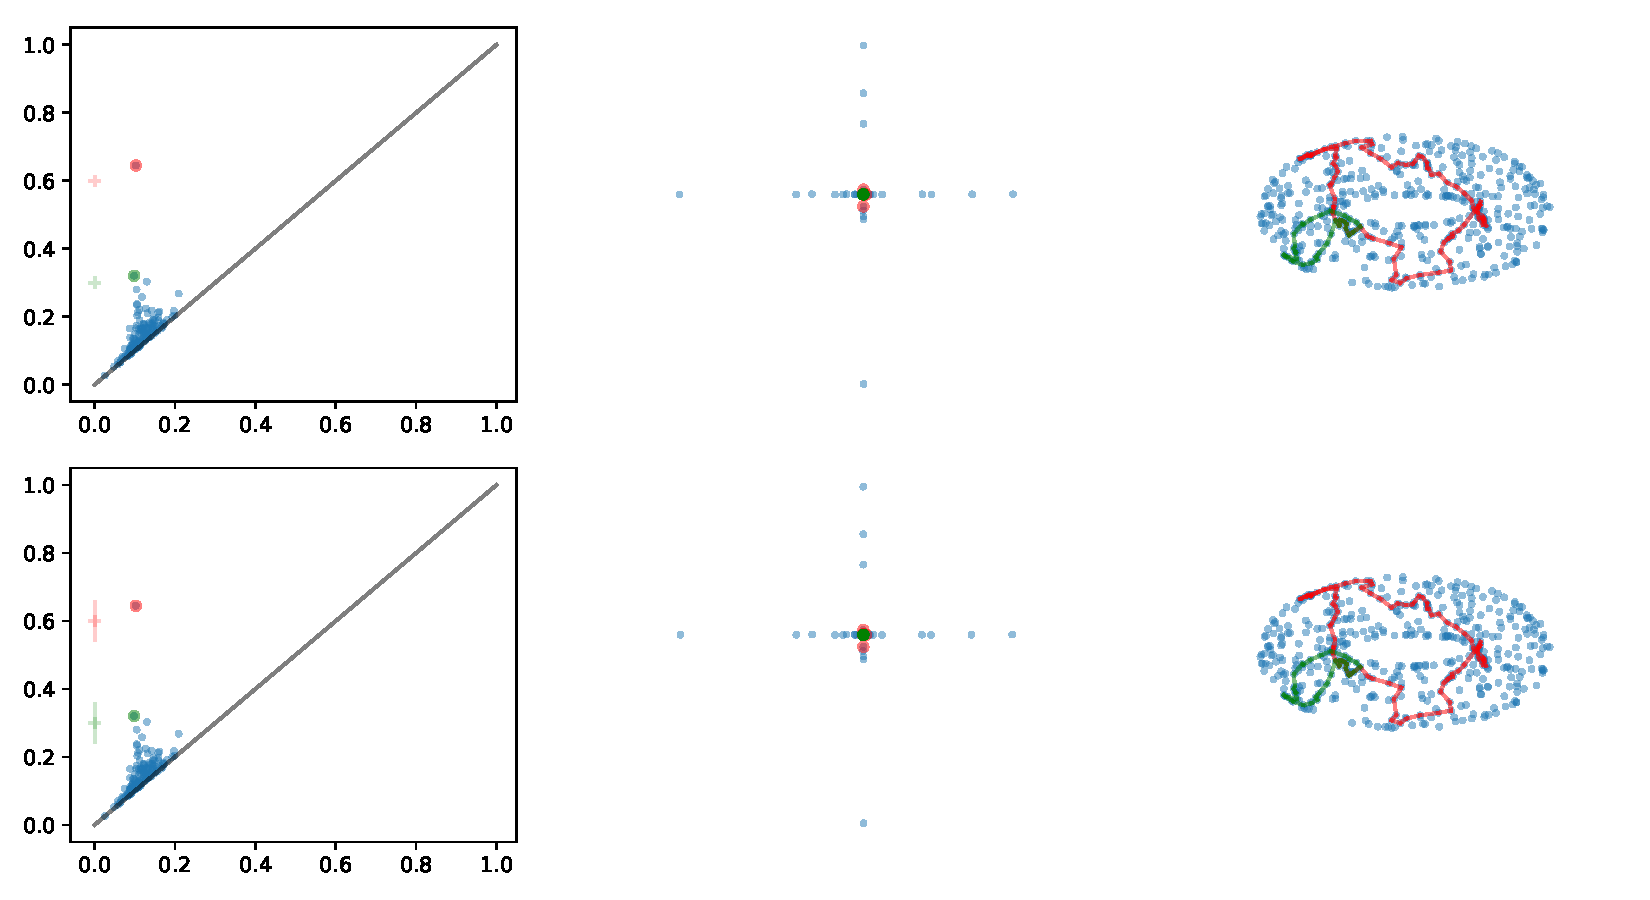
\includegraphics[width=\textwidth]{{figures/500random5.5}.pdf}
%         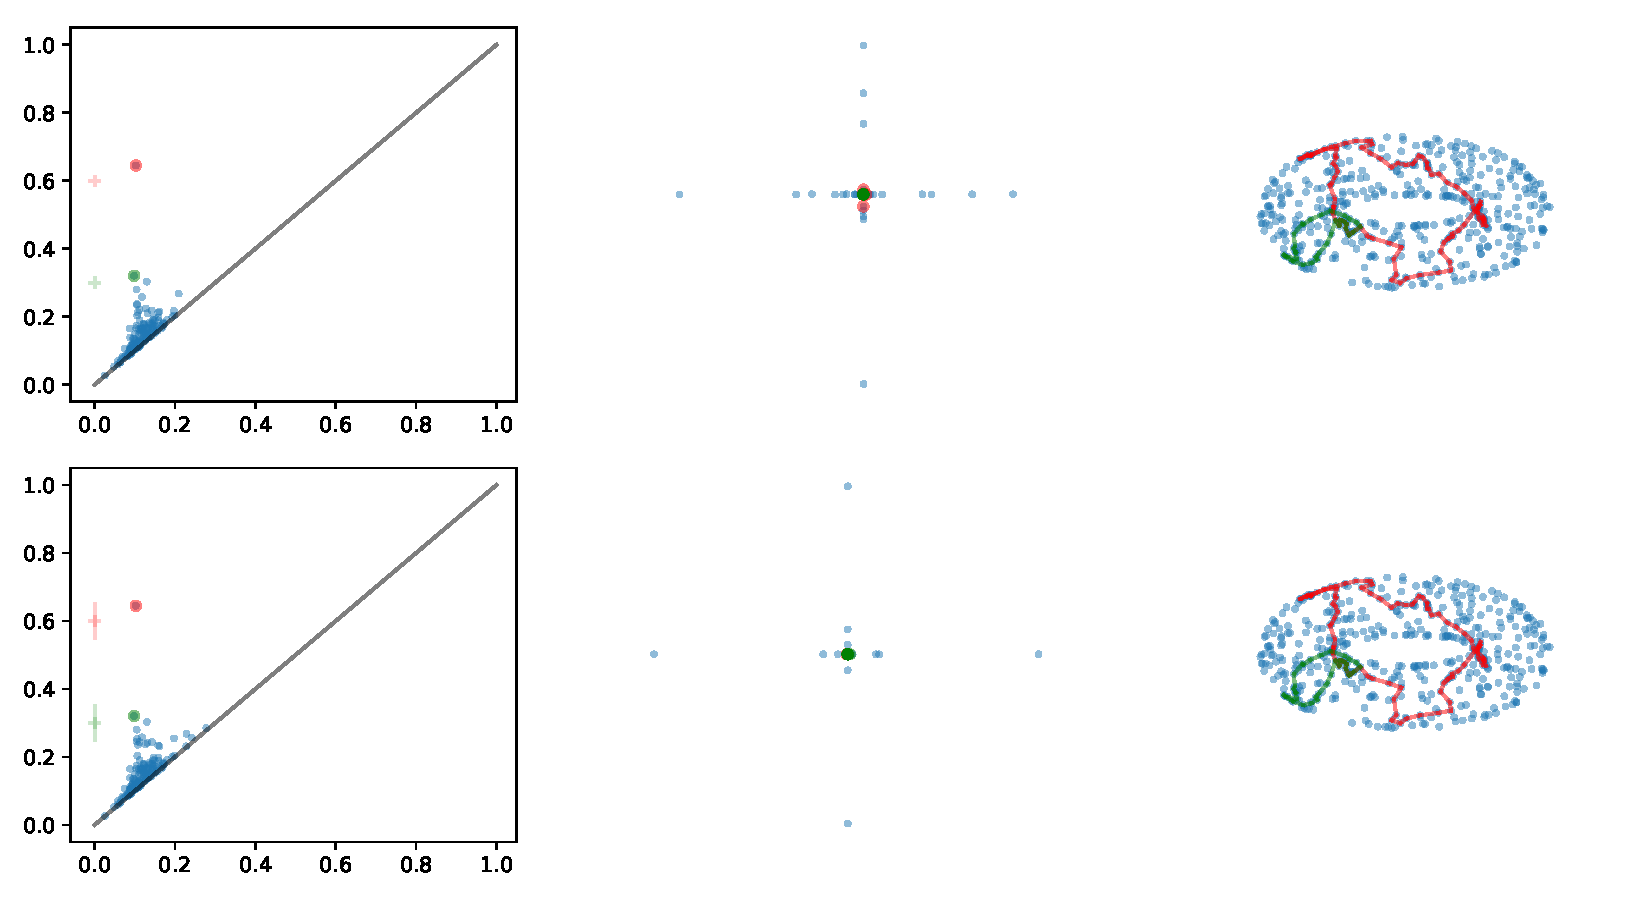
\includegraphics[width=\textwidth]{{figures/500random6.0}.pdf}
%         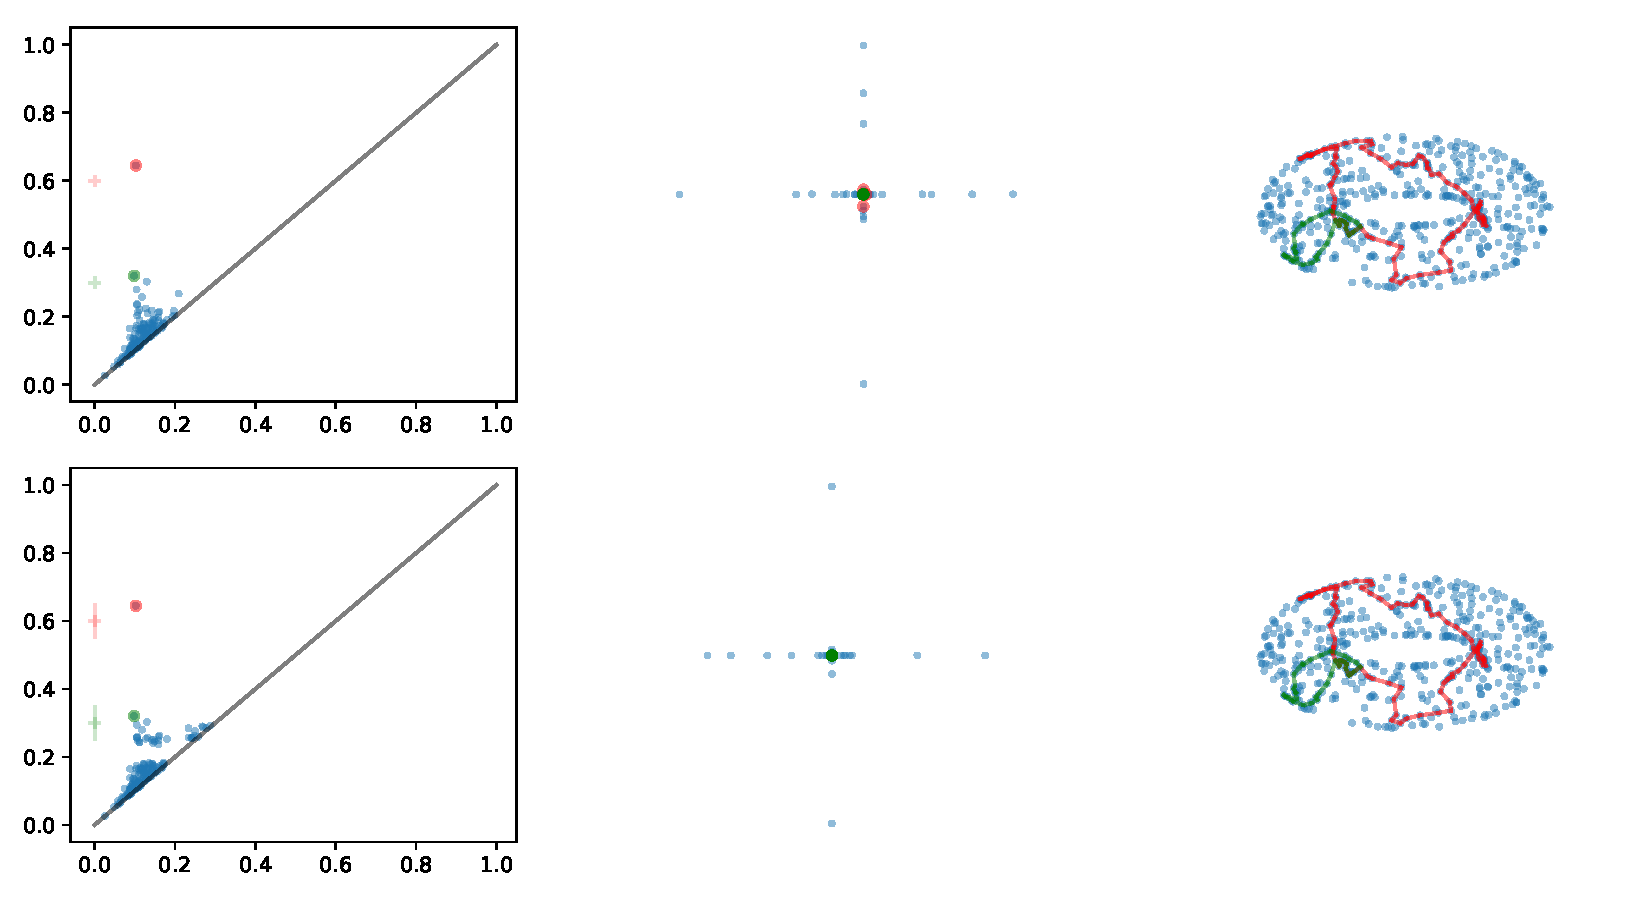
\includegraphics[width=\textwidth]{{figures/500random6.5}.pdf}
%         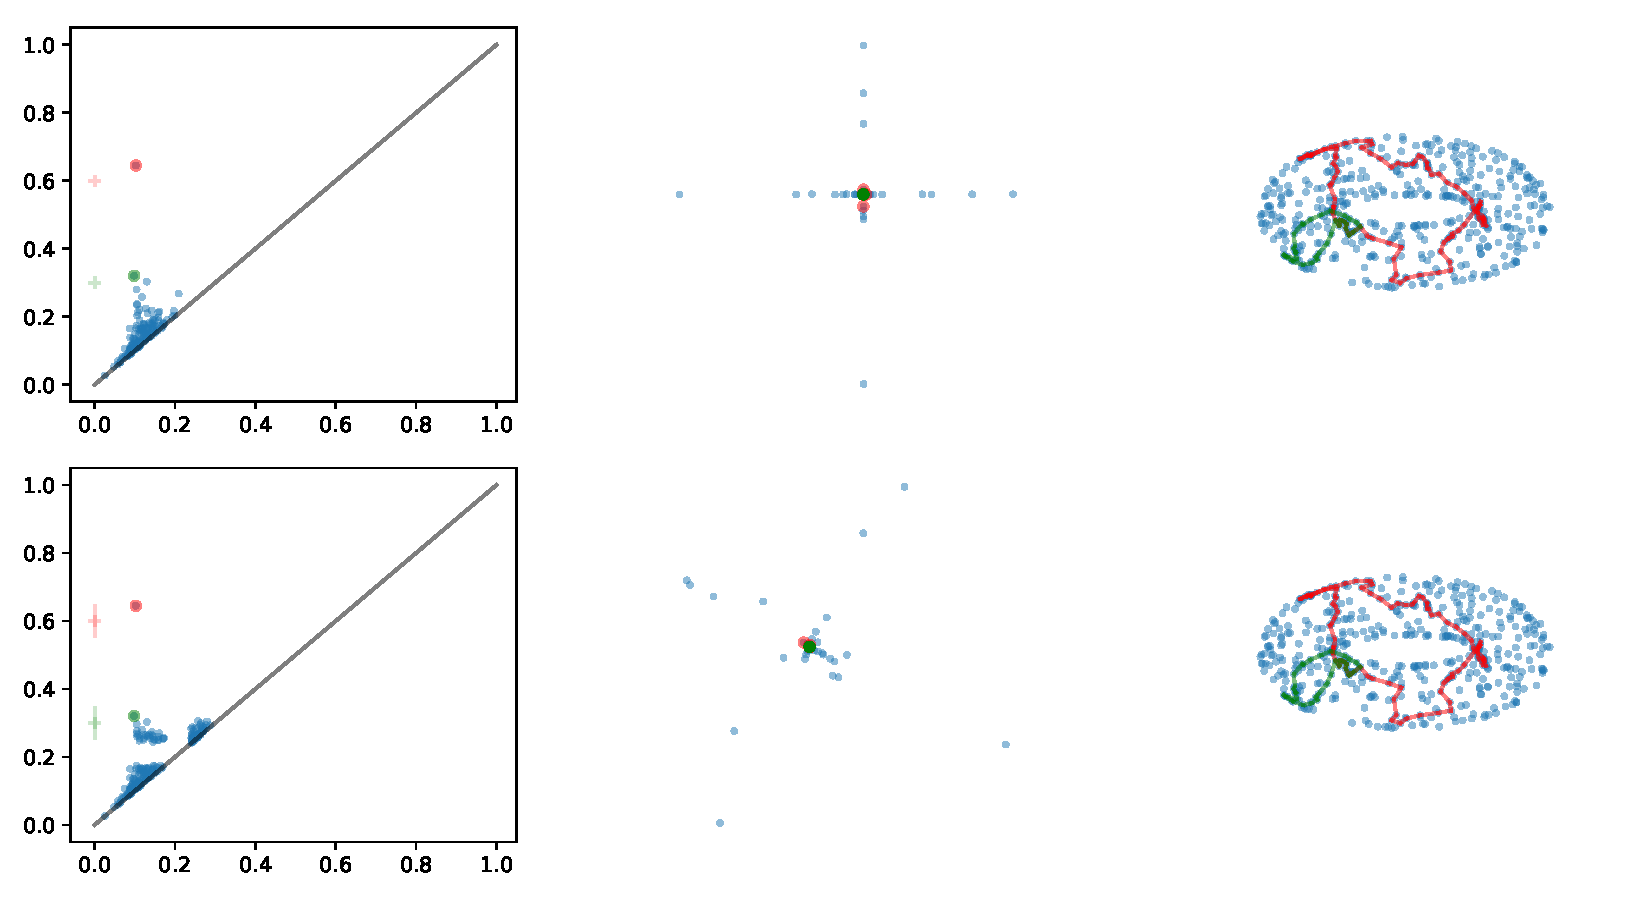
\includegraphics[width=\textwidth]{{figures/500random7.0}.pdf}
%         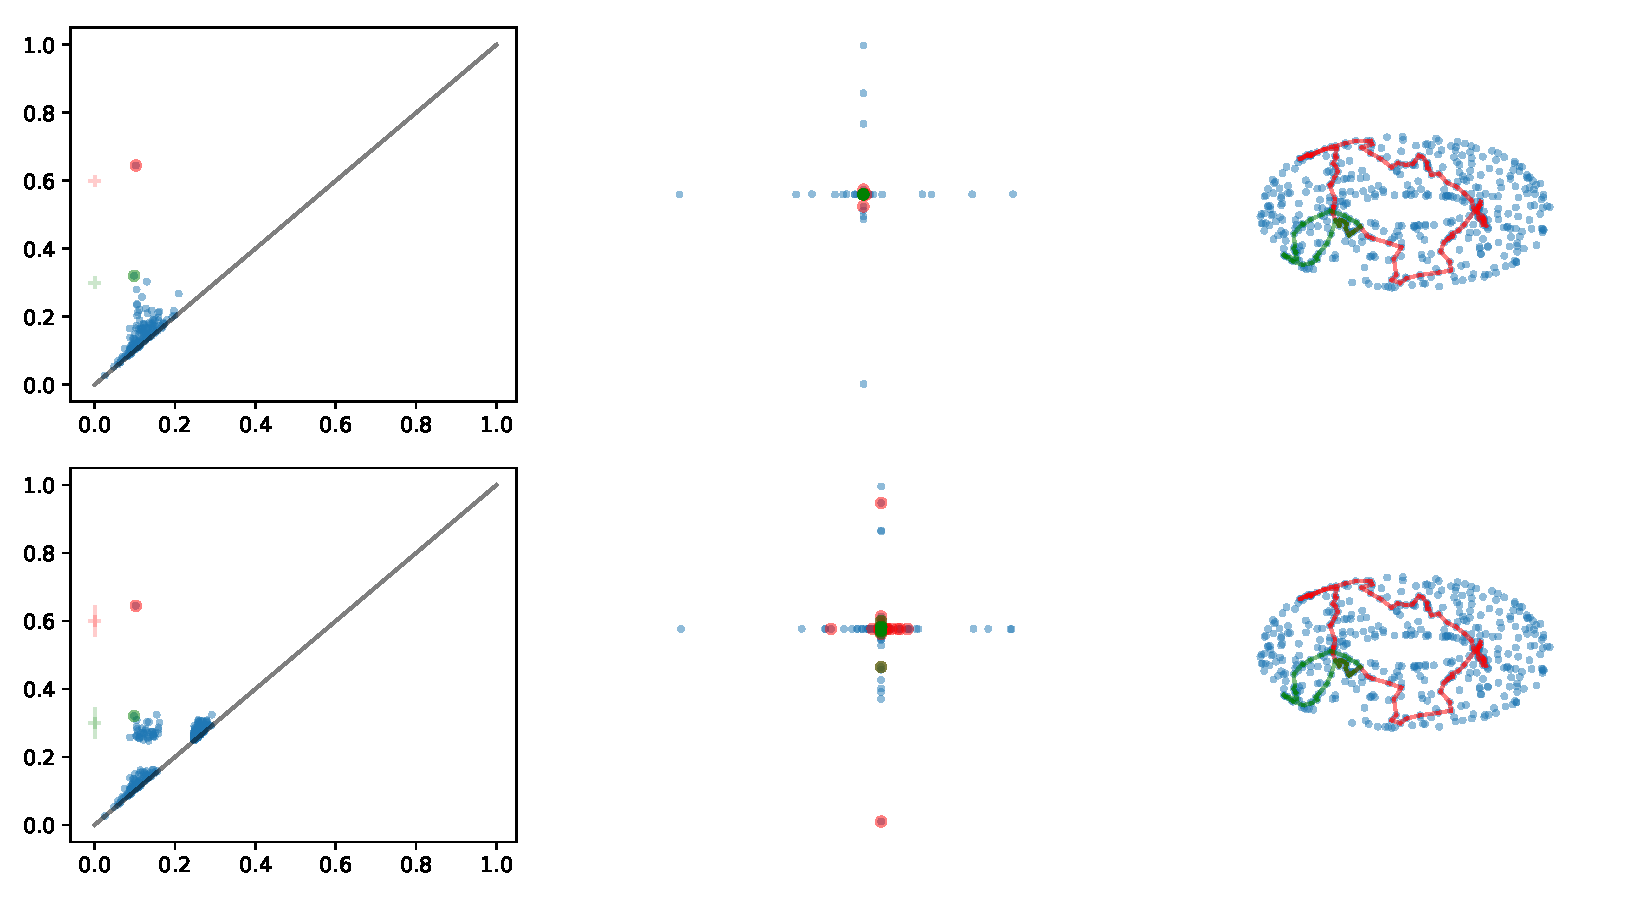
\includegraphics[width=\textwidth]{{figures/500random7.5}.pdf}
%         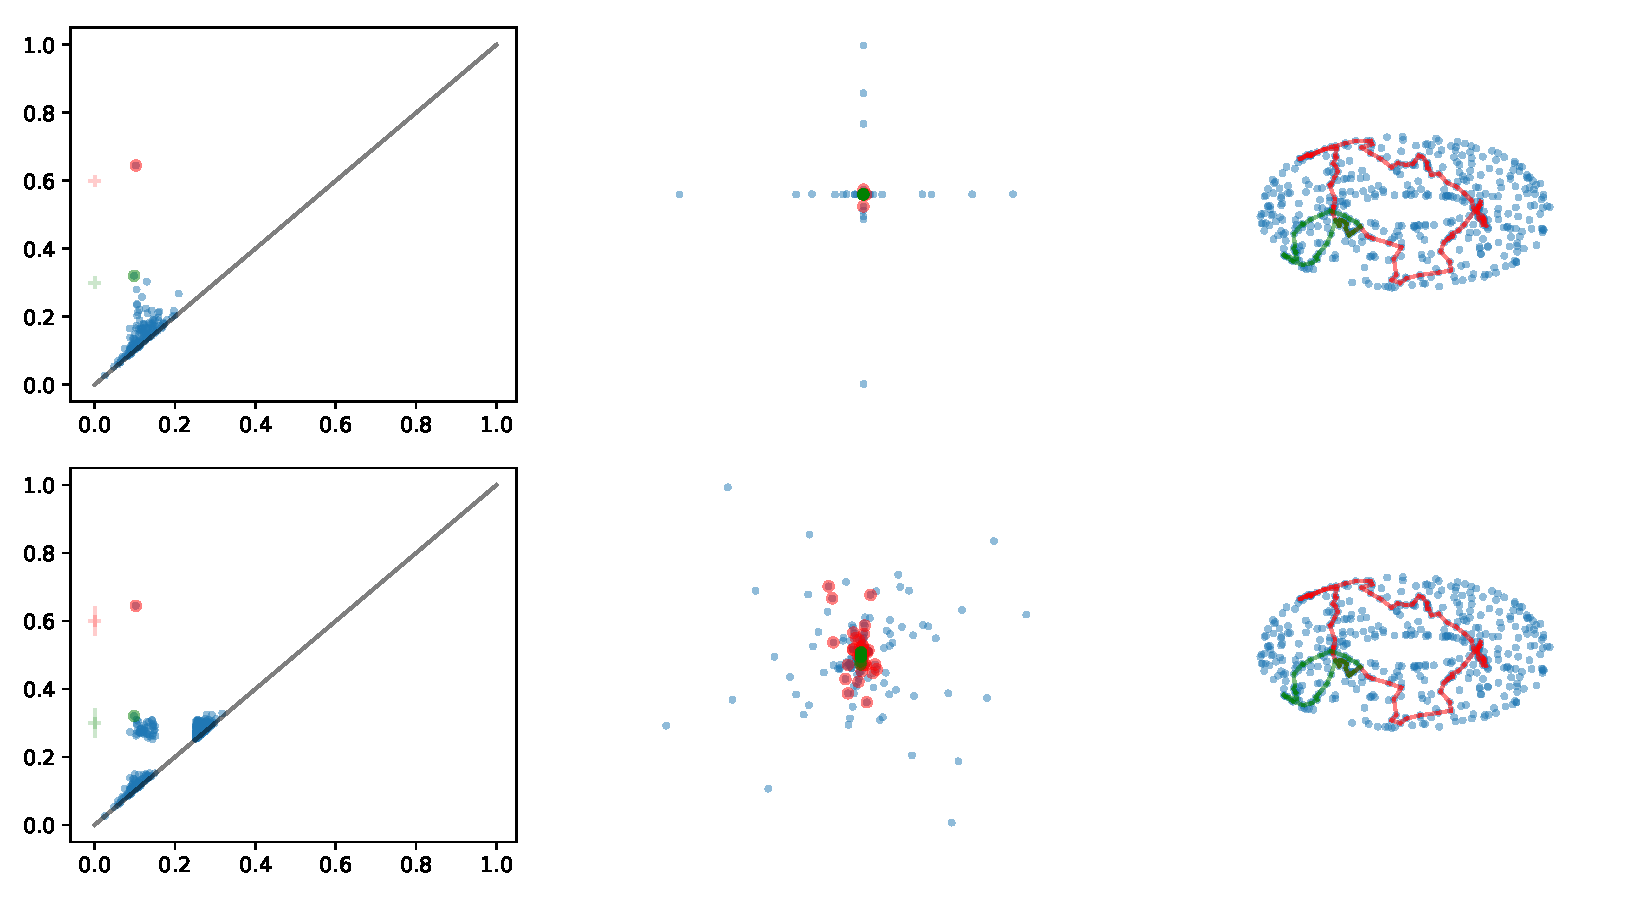
\includegraphics[width=\textwidth]{{figures/500random8.0}.pdf}
%         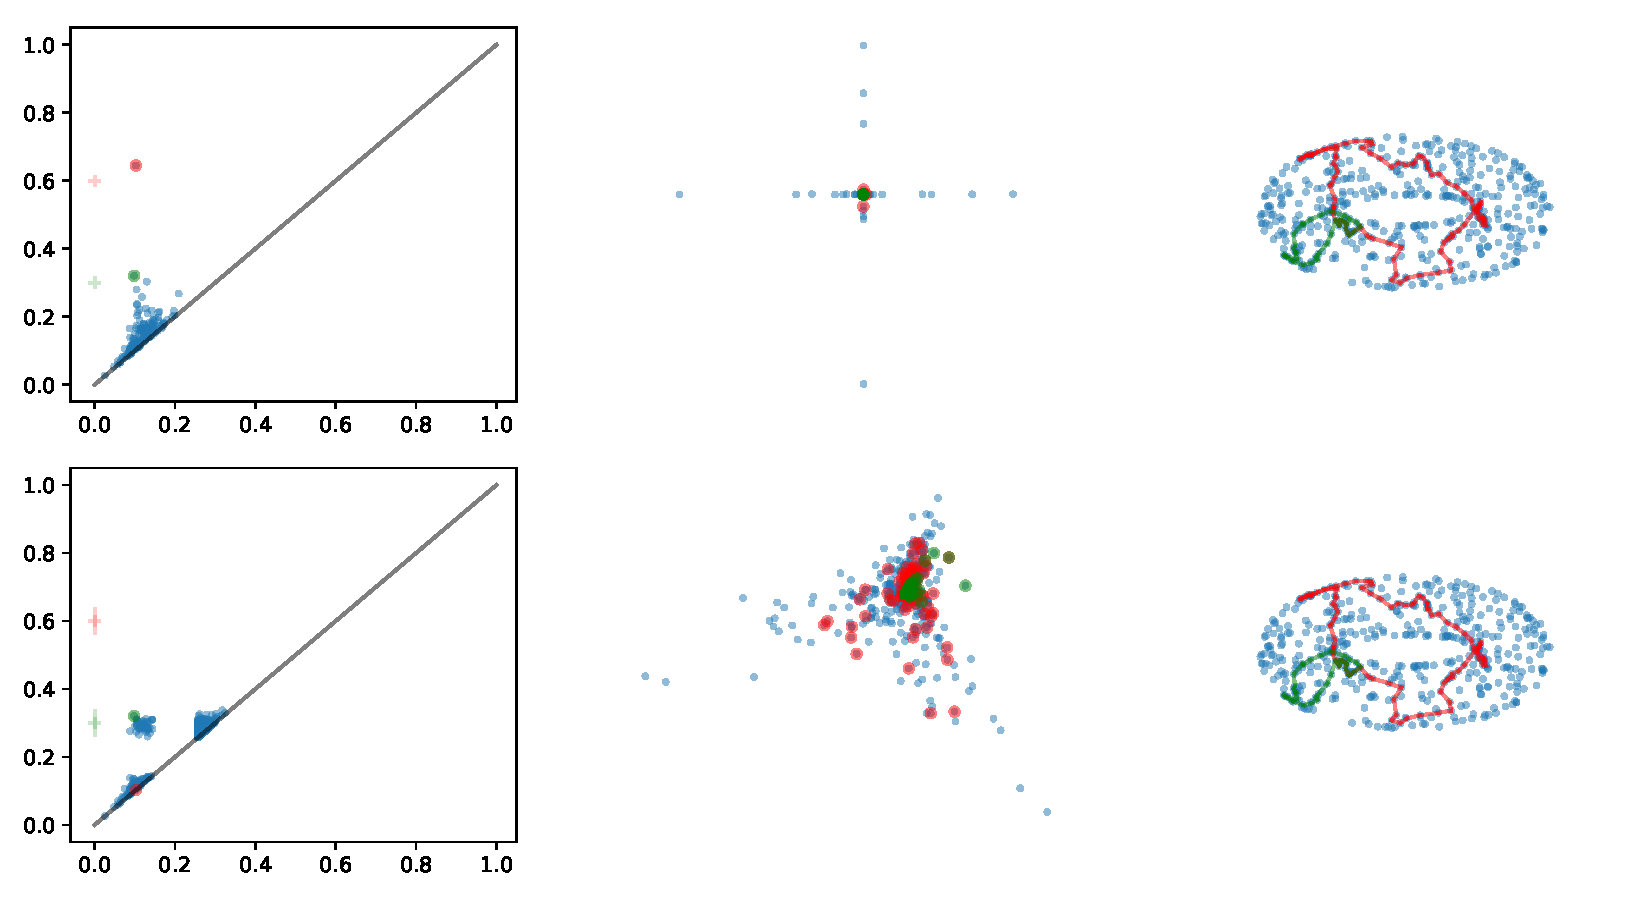
\includegraphics[width=\textwidth]{{figures/500random8.5}.pdf}
%         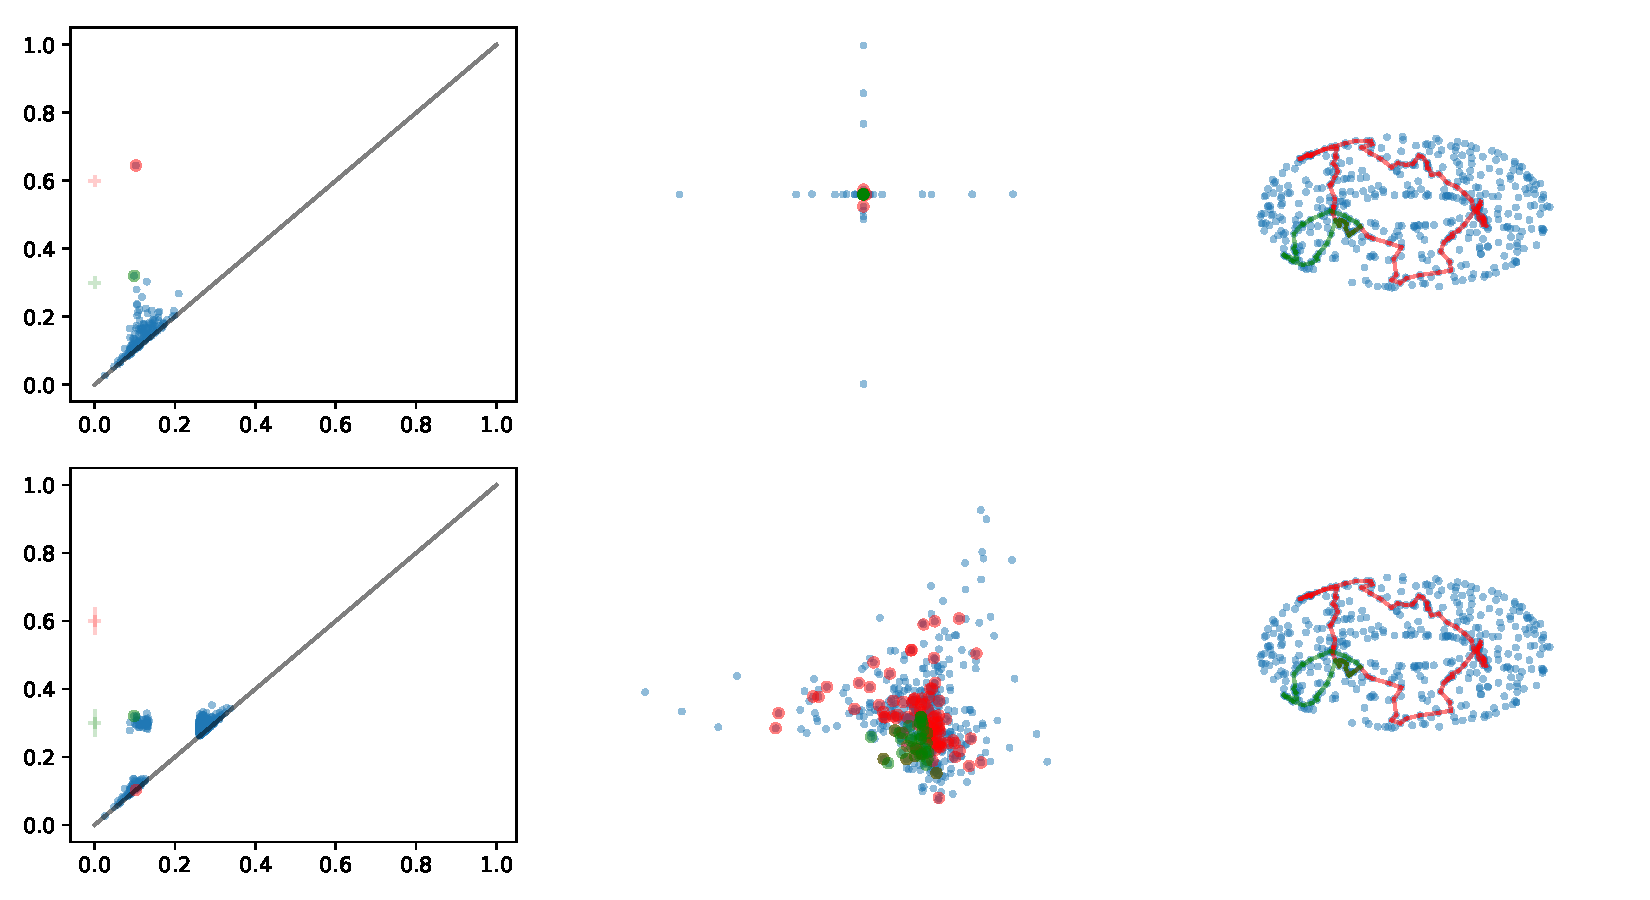
\includegraphics[width=\textwidth]{{figures/500random9.0}.pdf}
%         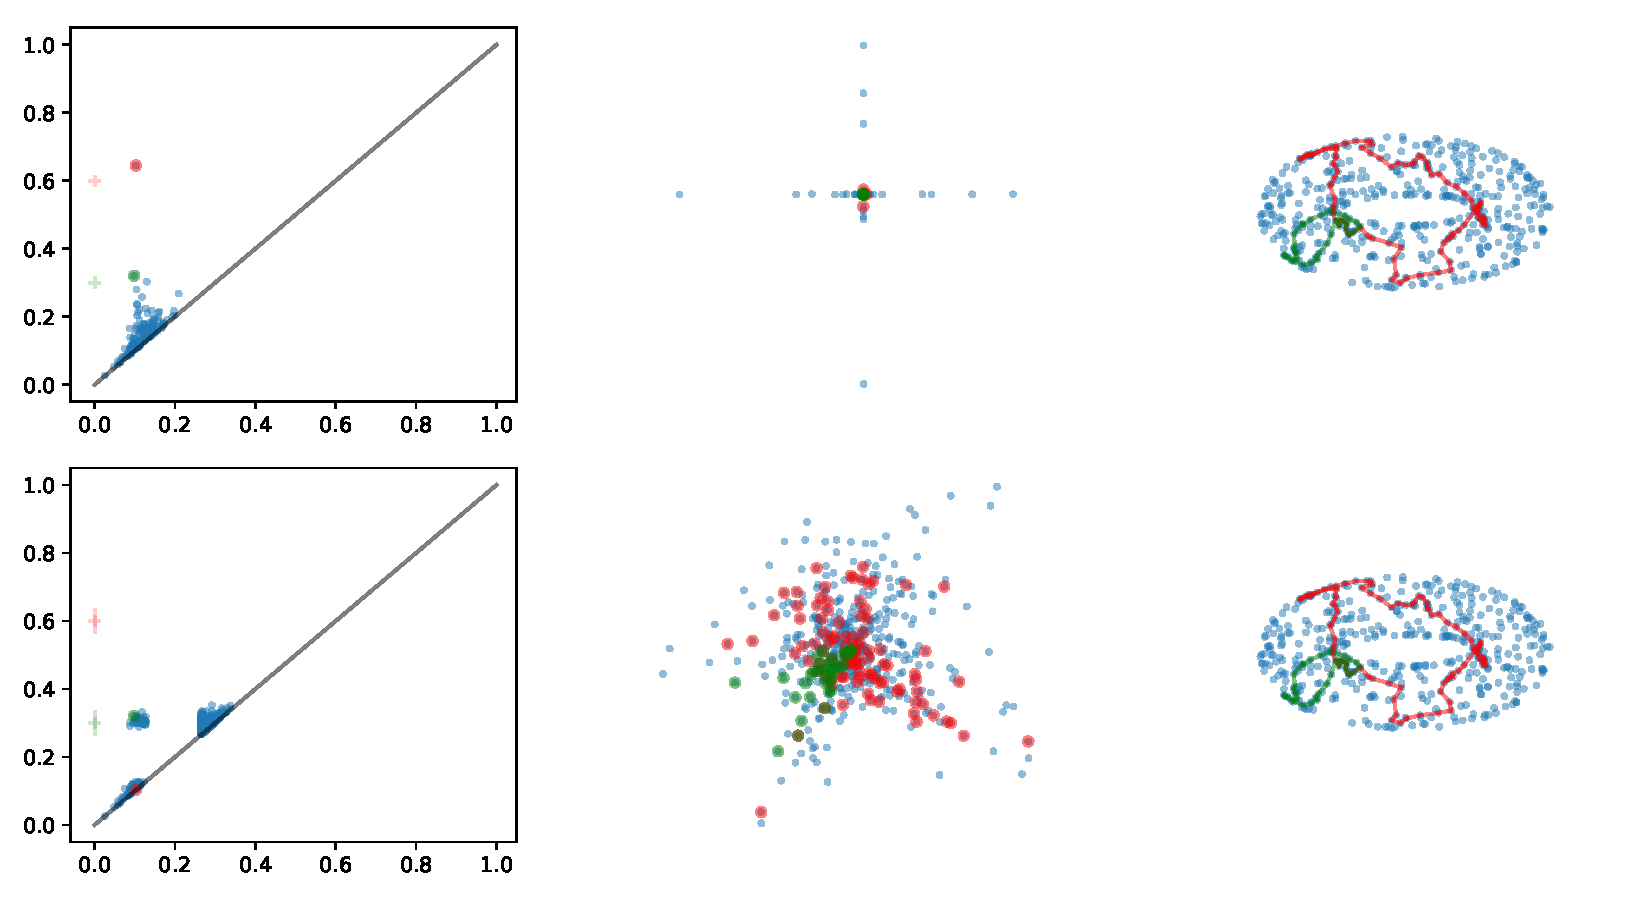
\includegraphics[width=\textwidth]{{figures/500random9.5}.pdf}
%         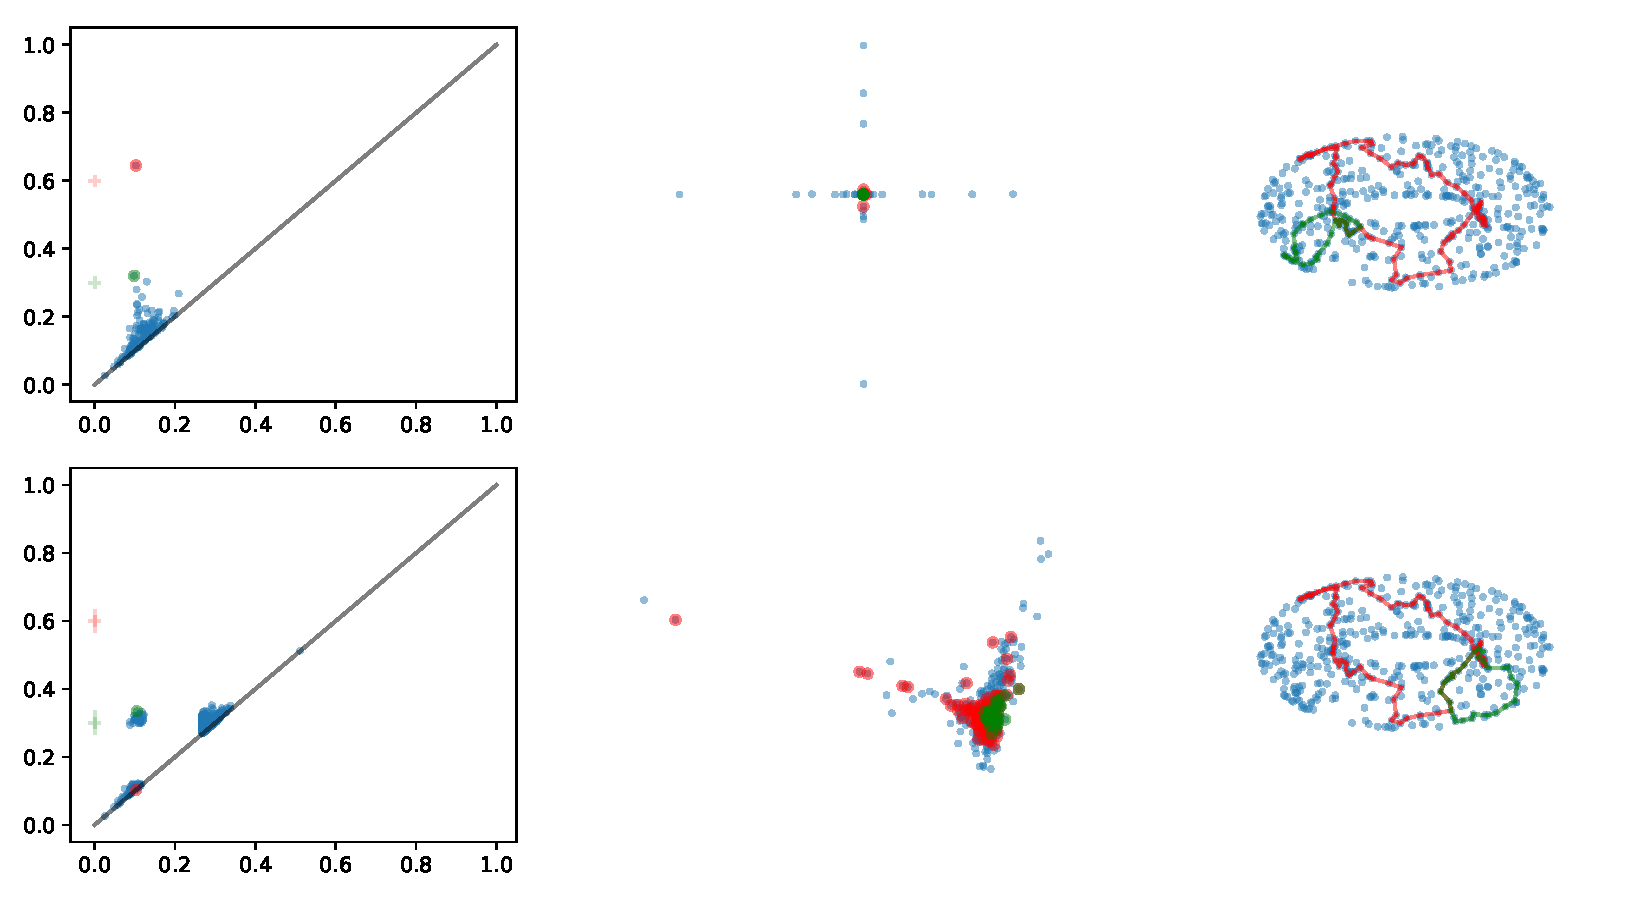
\includegraphics[width=\textwidth]{{figures/500random10.0}.pdf}
%         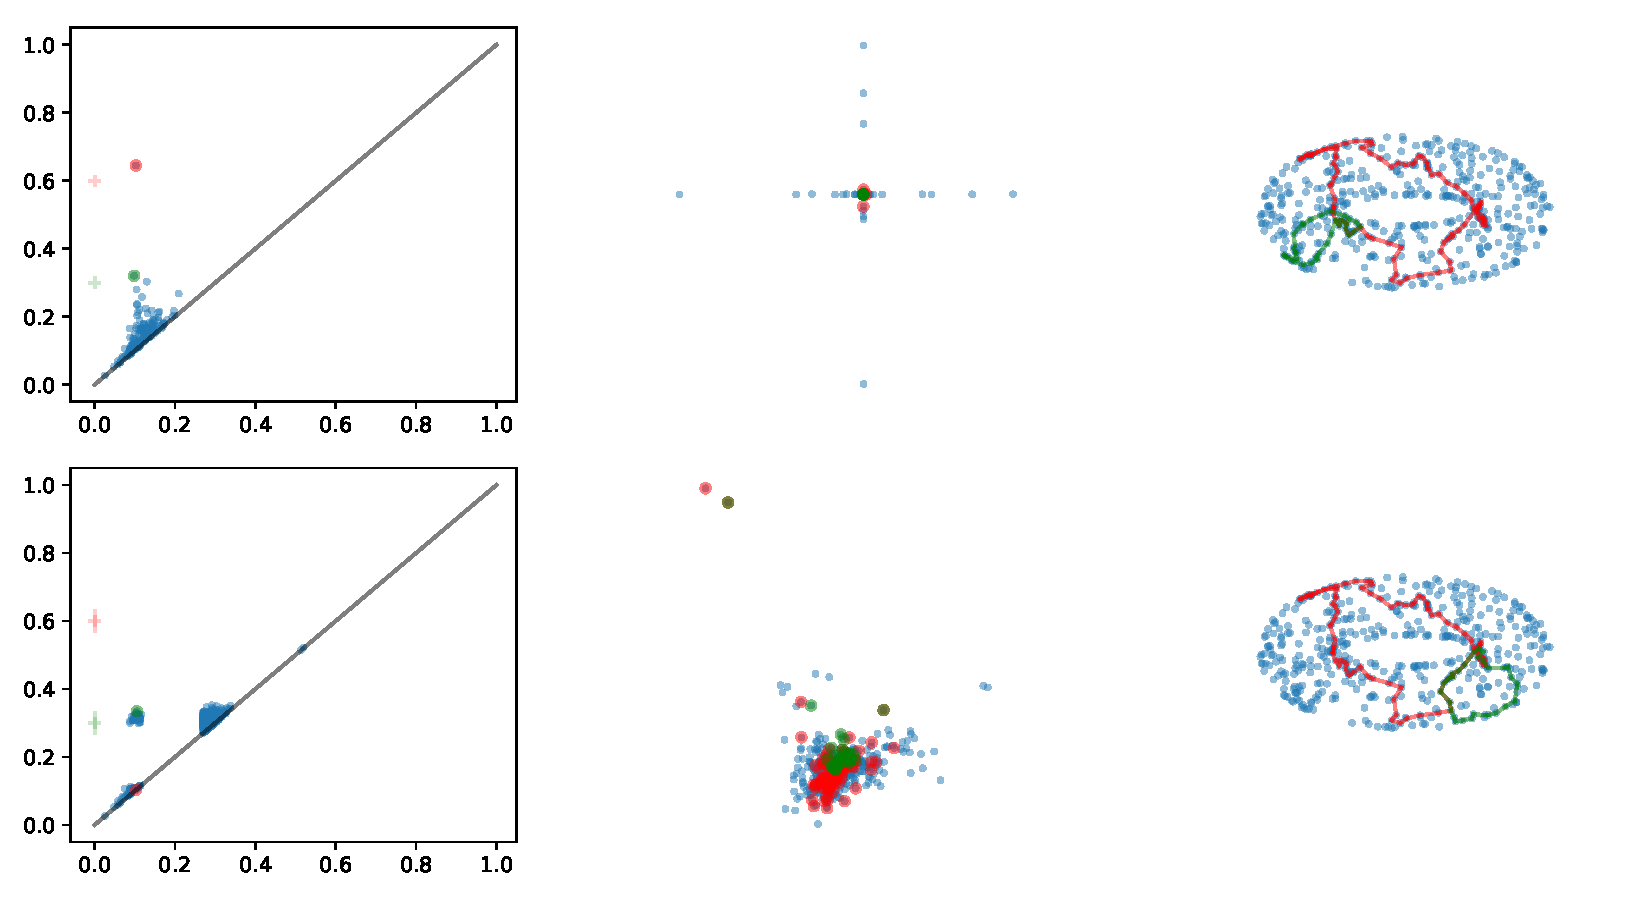
\includegraphics[width=\textwidth]{{figures/500random10.5}.pdf}
%         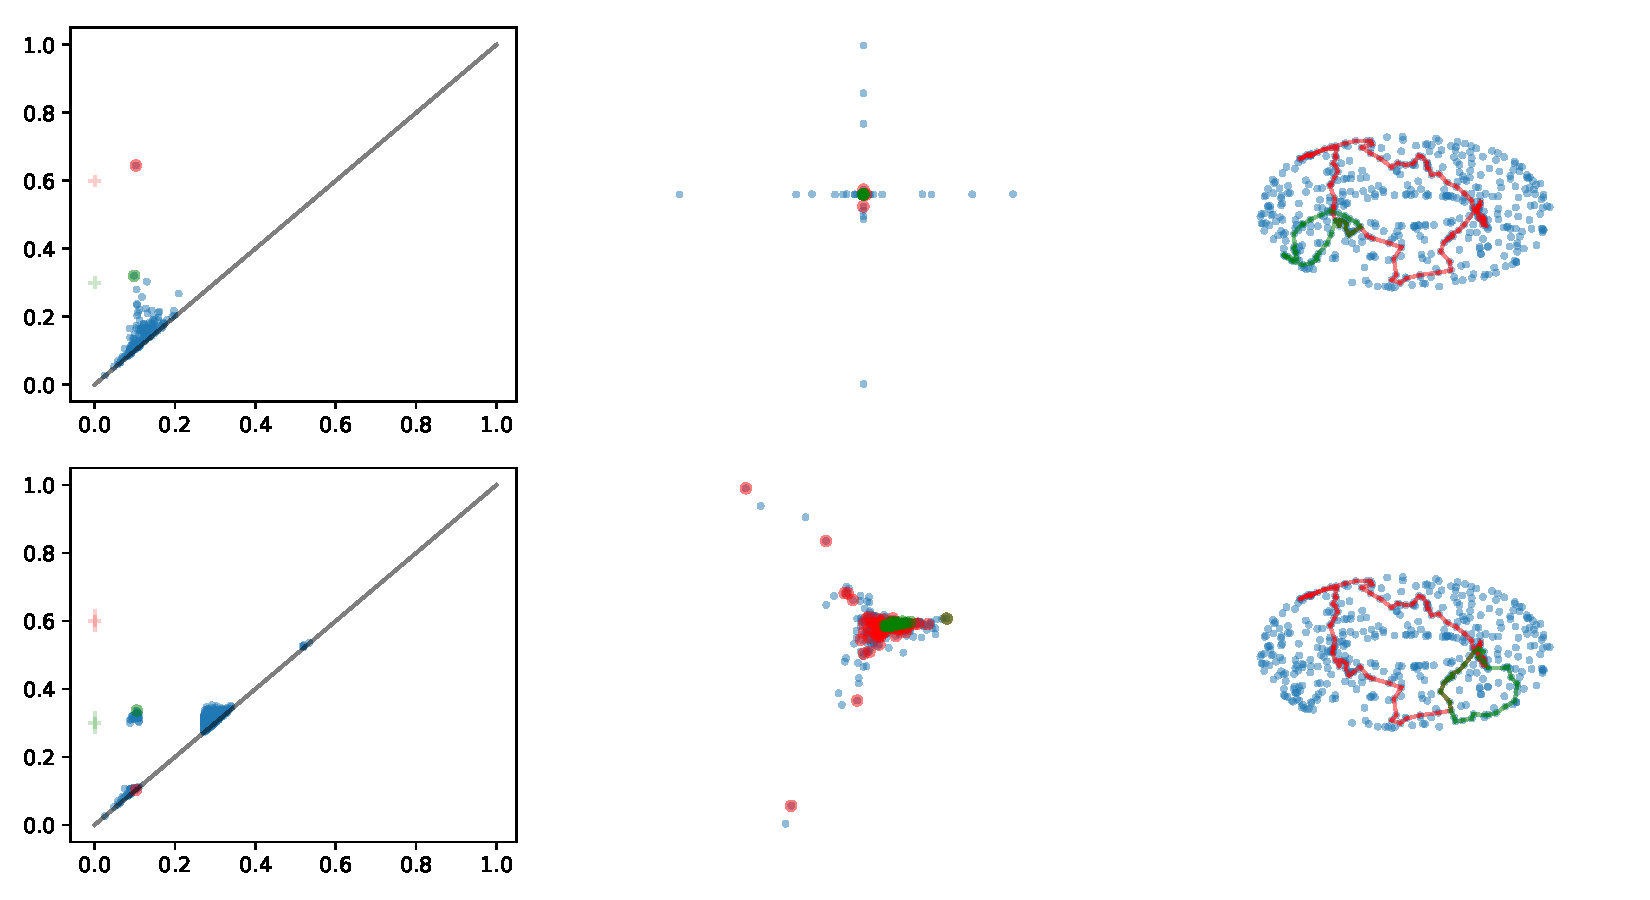
\includegraphics[width=\textwidth]{{figures/500random11.0}.pdf}
%         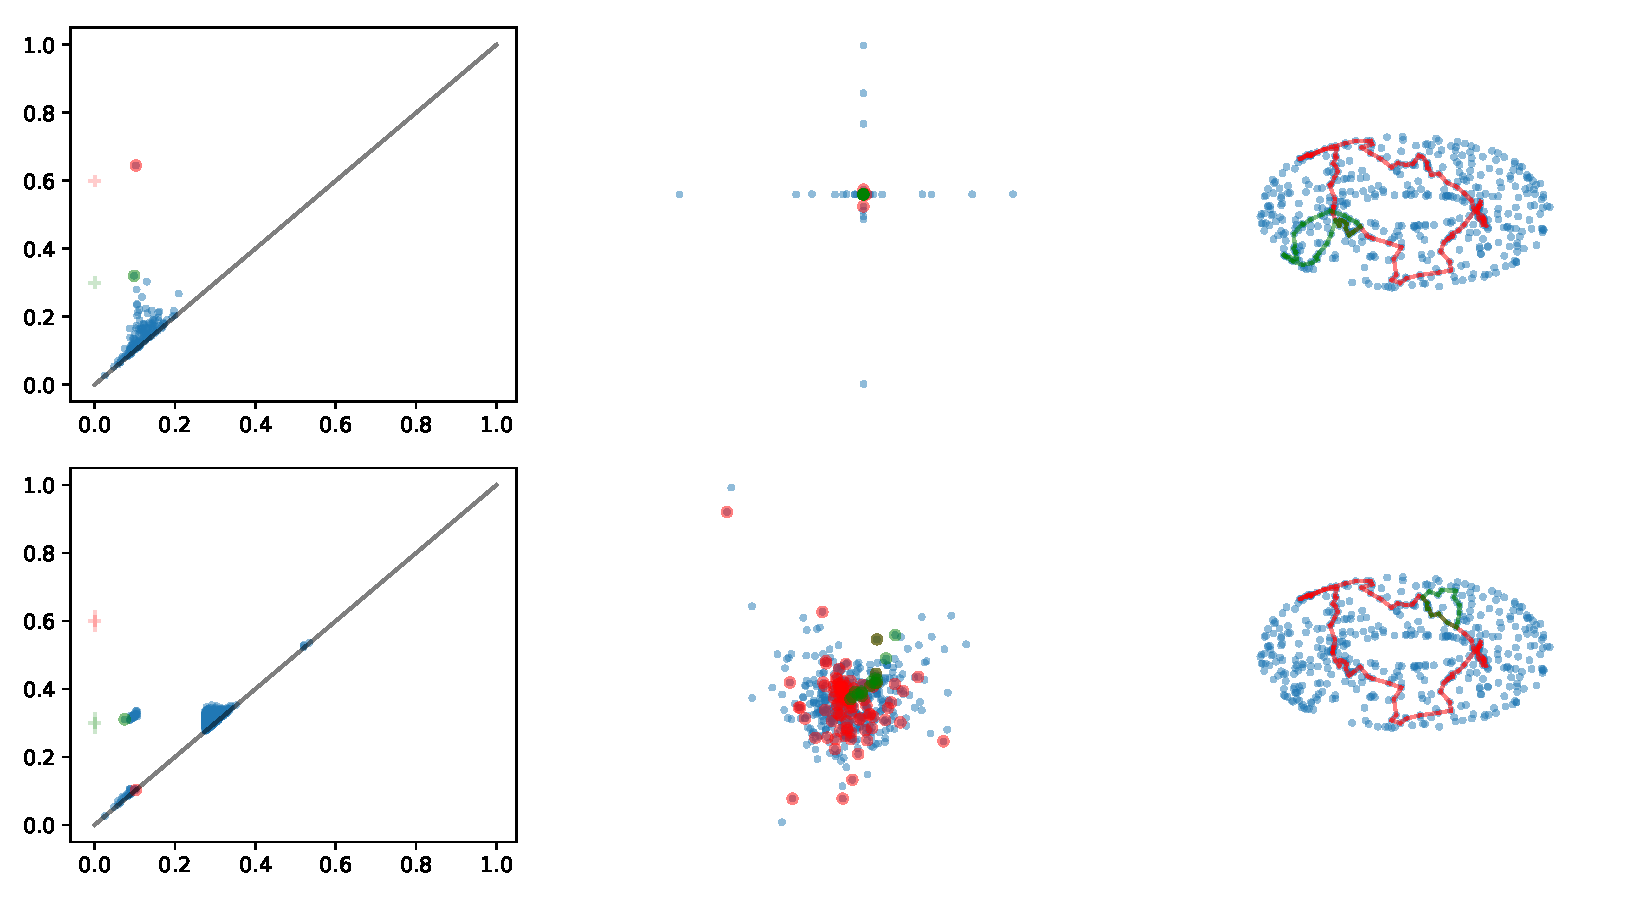
\includegraphics[width=\textwidth]{{figures/500random11.5}.pdf}
%         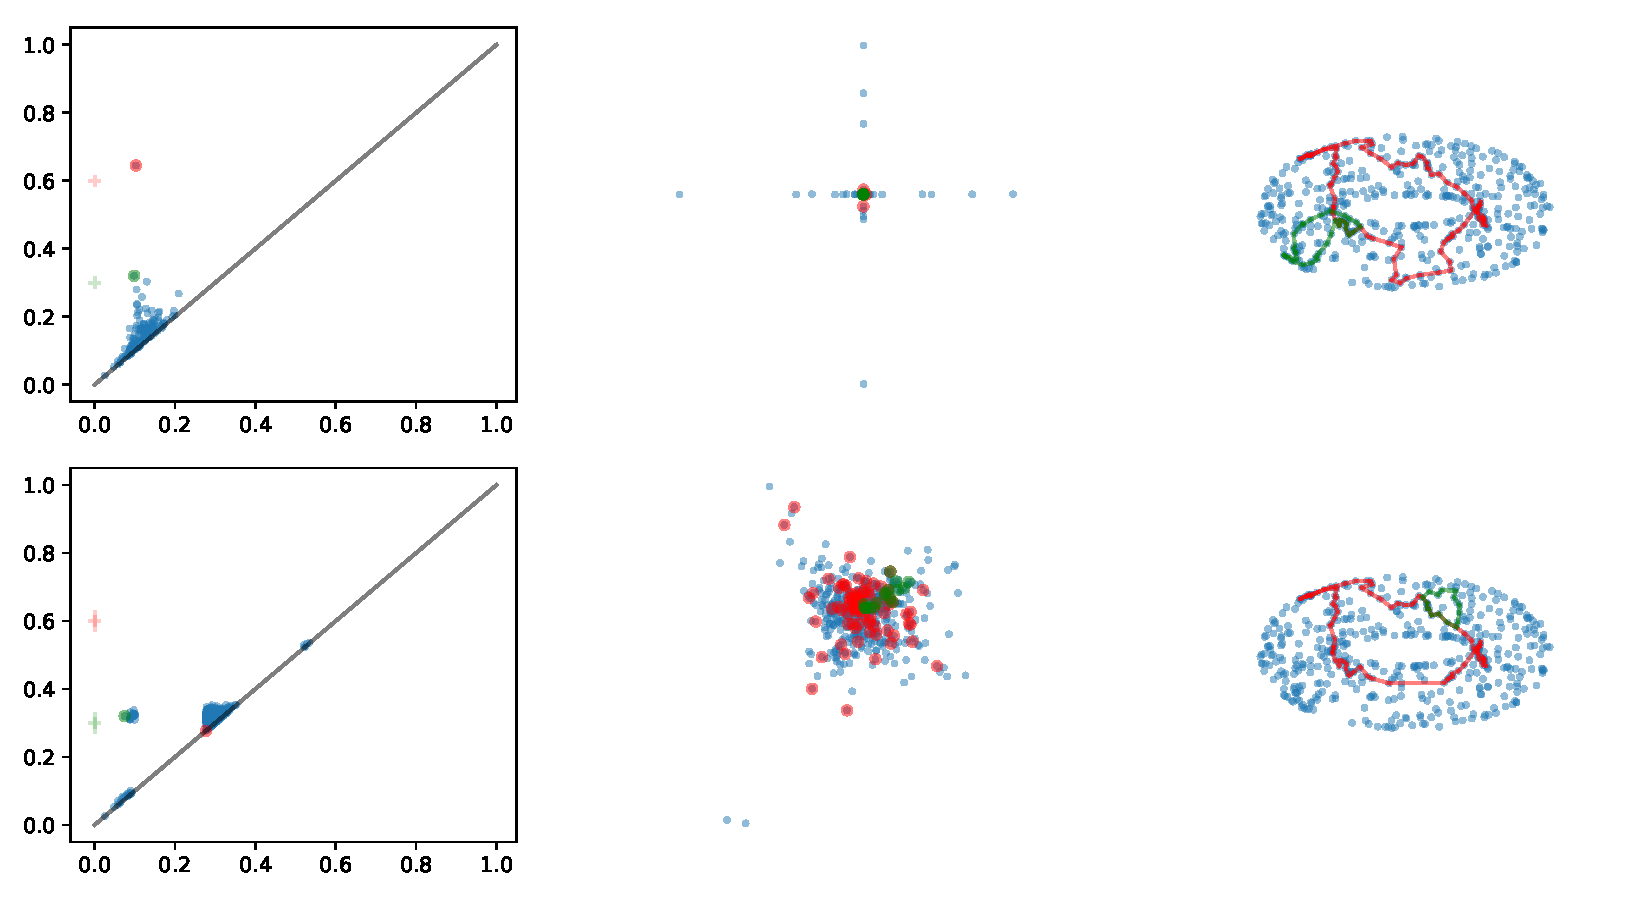
\includegraphics[width=\textwidth]{{figures/500random12.0}.pdf}
%         % \caption{}\label{fig:mdss}
% \end{figure}

\end{document}
